\chapter{Game theoretic model - Numerical results}
\label{appendix:game_theoretic_model}

Appendix~\ref{appendix:game_theoretic_model} contains additional numerical
results for the game theoretic model presented in
Chapter~\ref{sec:game_theoretic_model}.
These results build on the results presented in
Chapter~\ref{sec:numerical_results} and were omitted from the main text for
brevity.

This appendix presents additional results of the asymmetric replicator dynamics
run and PoA of the game theoretic model with different time targets and
multiple values of the ``weight'' parameter.
Refer to Chapter~\ref{sec:numerical_results} for a description of the
asymmetric replicator dynamics run and PoA metrics.
Section~\ref{app:b_1} shows some runs of the asymmetric replicator dynamics
while changing the value of the time target parameter \(t\).
Section~\ref{app:b_2} presents a different set of runs of the asymmetric
replicator dynamics while changing the value of the ``weight'' parameter
\(\alpha\).
Finally, Section~\ref{app:b_3} shows the results of the game theoretic model
for some other custom values of the parameters. 


\section{Changing time targets}\label{app:b_1}

\begin{figure}[H]
    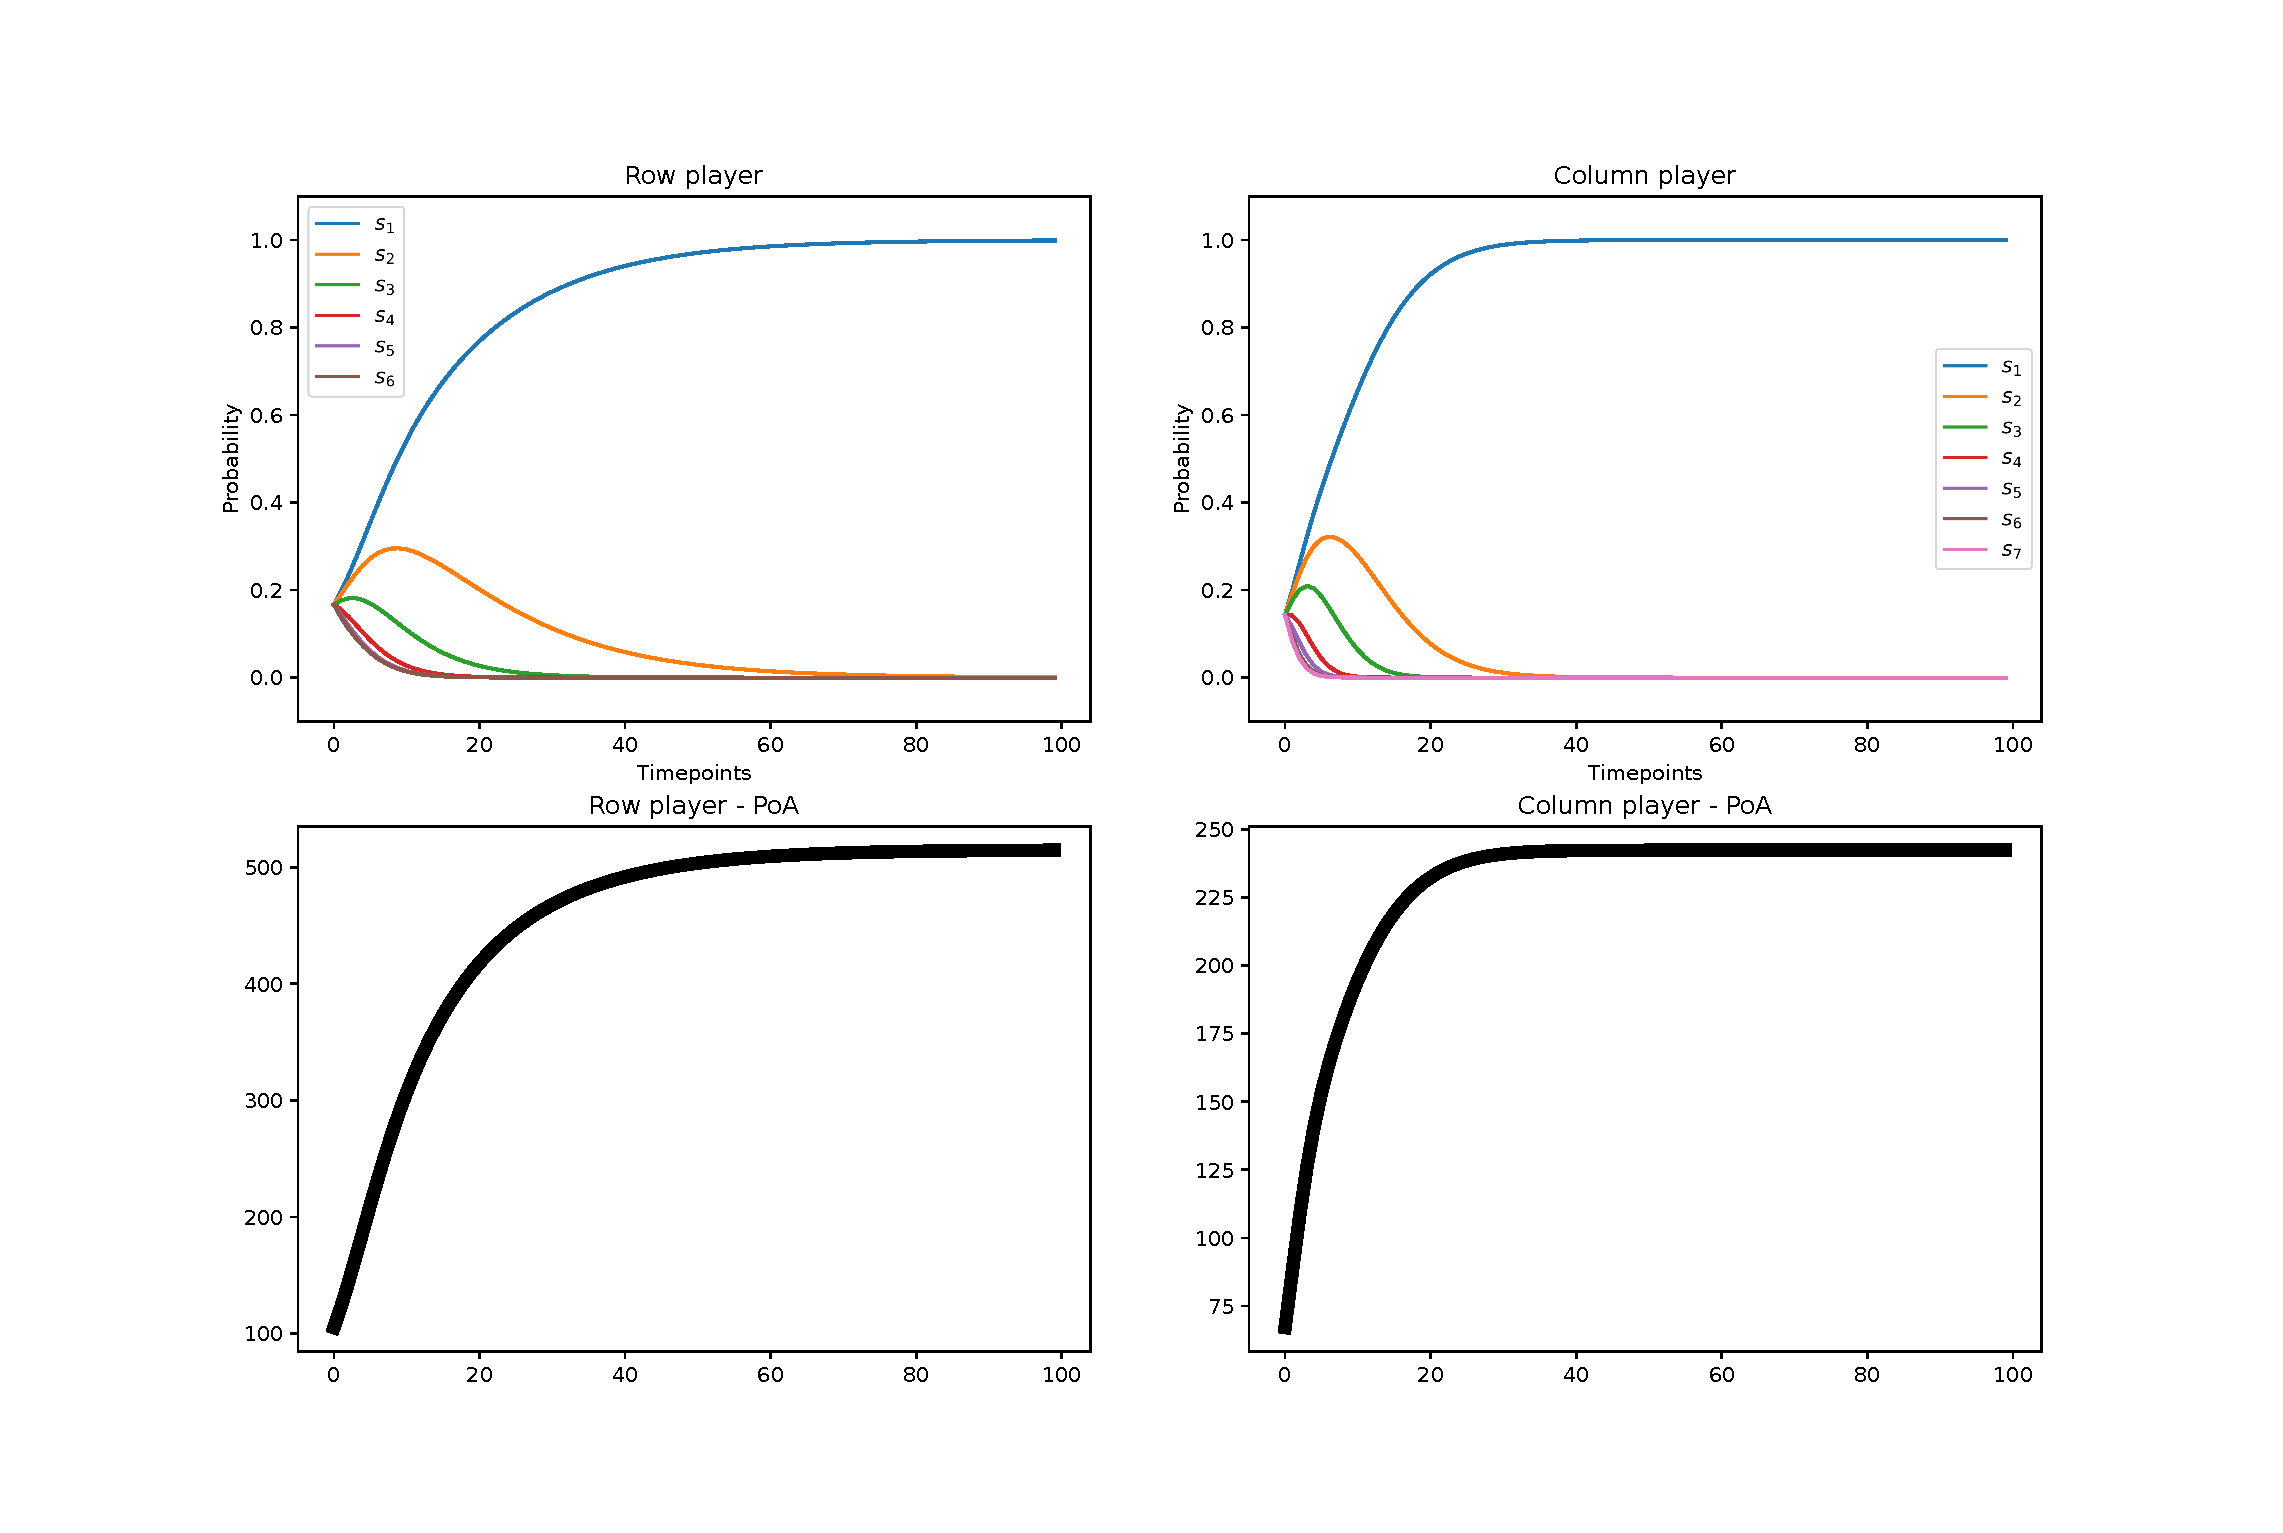
\includegraphics[width=\textwidth, trim = 0 60 0 60, clip]{chapters/00_appendix/02_more_game_results/Bin/poa_ard_target_1.eps}
    \caption{Asymmetric replicator dynamics run and PoA of the game theoretic
    model with time target 1.0 and parameters: \(\alpha = 0.97,
    \lambda_2 = 0.1, \lambda_1^{(1)} = 3.0, \lambda_1^{(2)} = 4.5,
    \mu^{(1)} = 2.0, \mu^{(2)} = 3.0, C^{(1)} = 3, C^{(2)} = 2,
    N^{(1)} = 6, N^{(2)} = 7, M^{(1)} = 5, M^{(2)} = 4\).}
    \label{fig:poa_ard_target_1}
\end{figure}


\begin{figure}[H]
    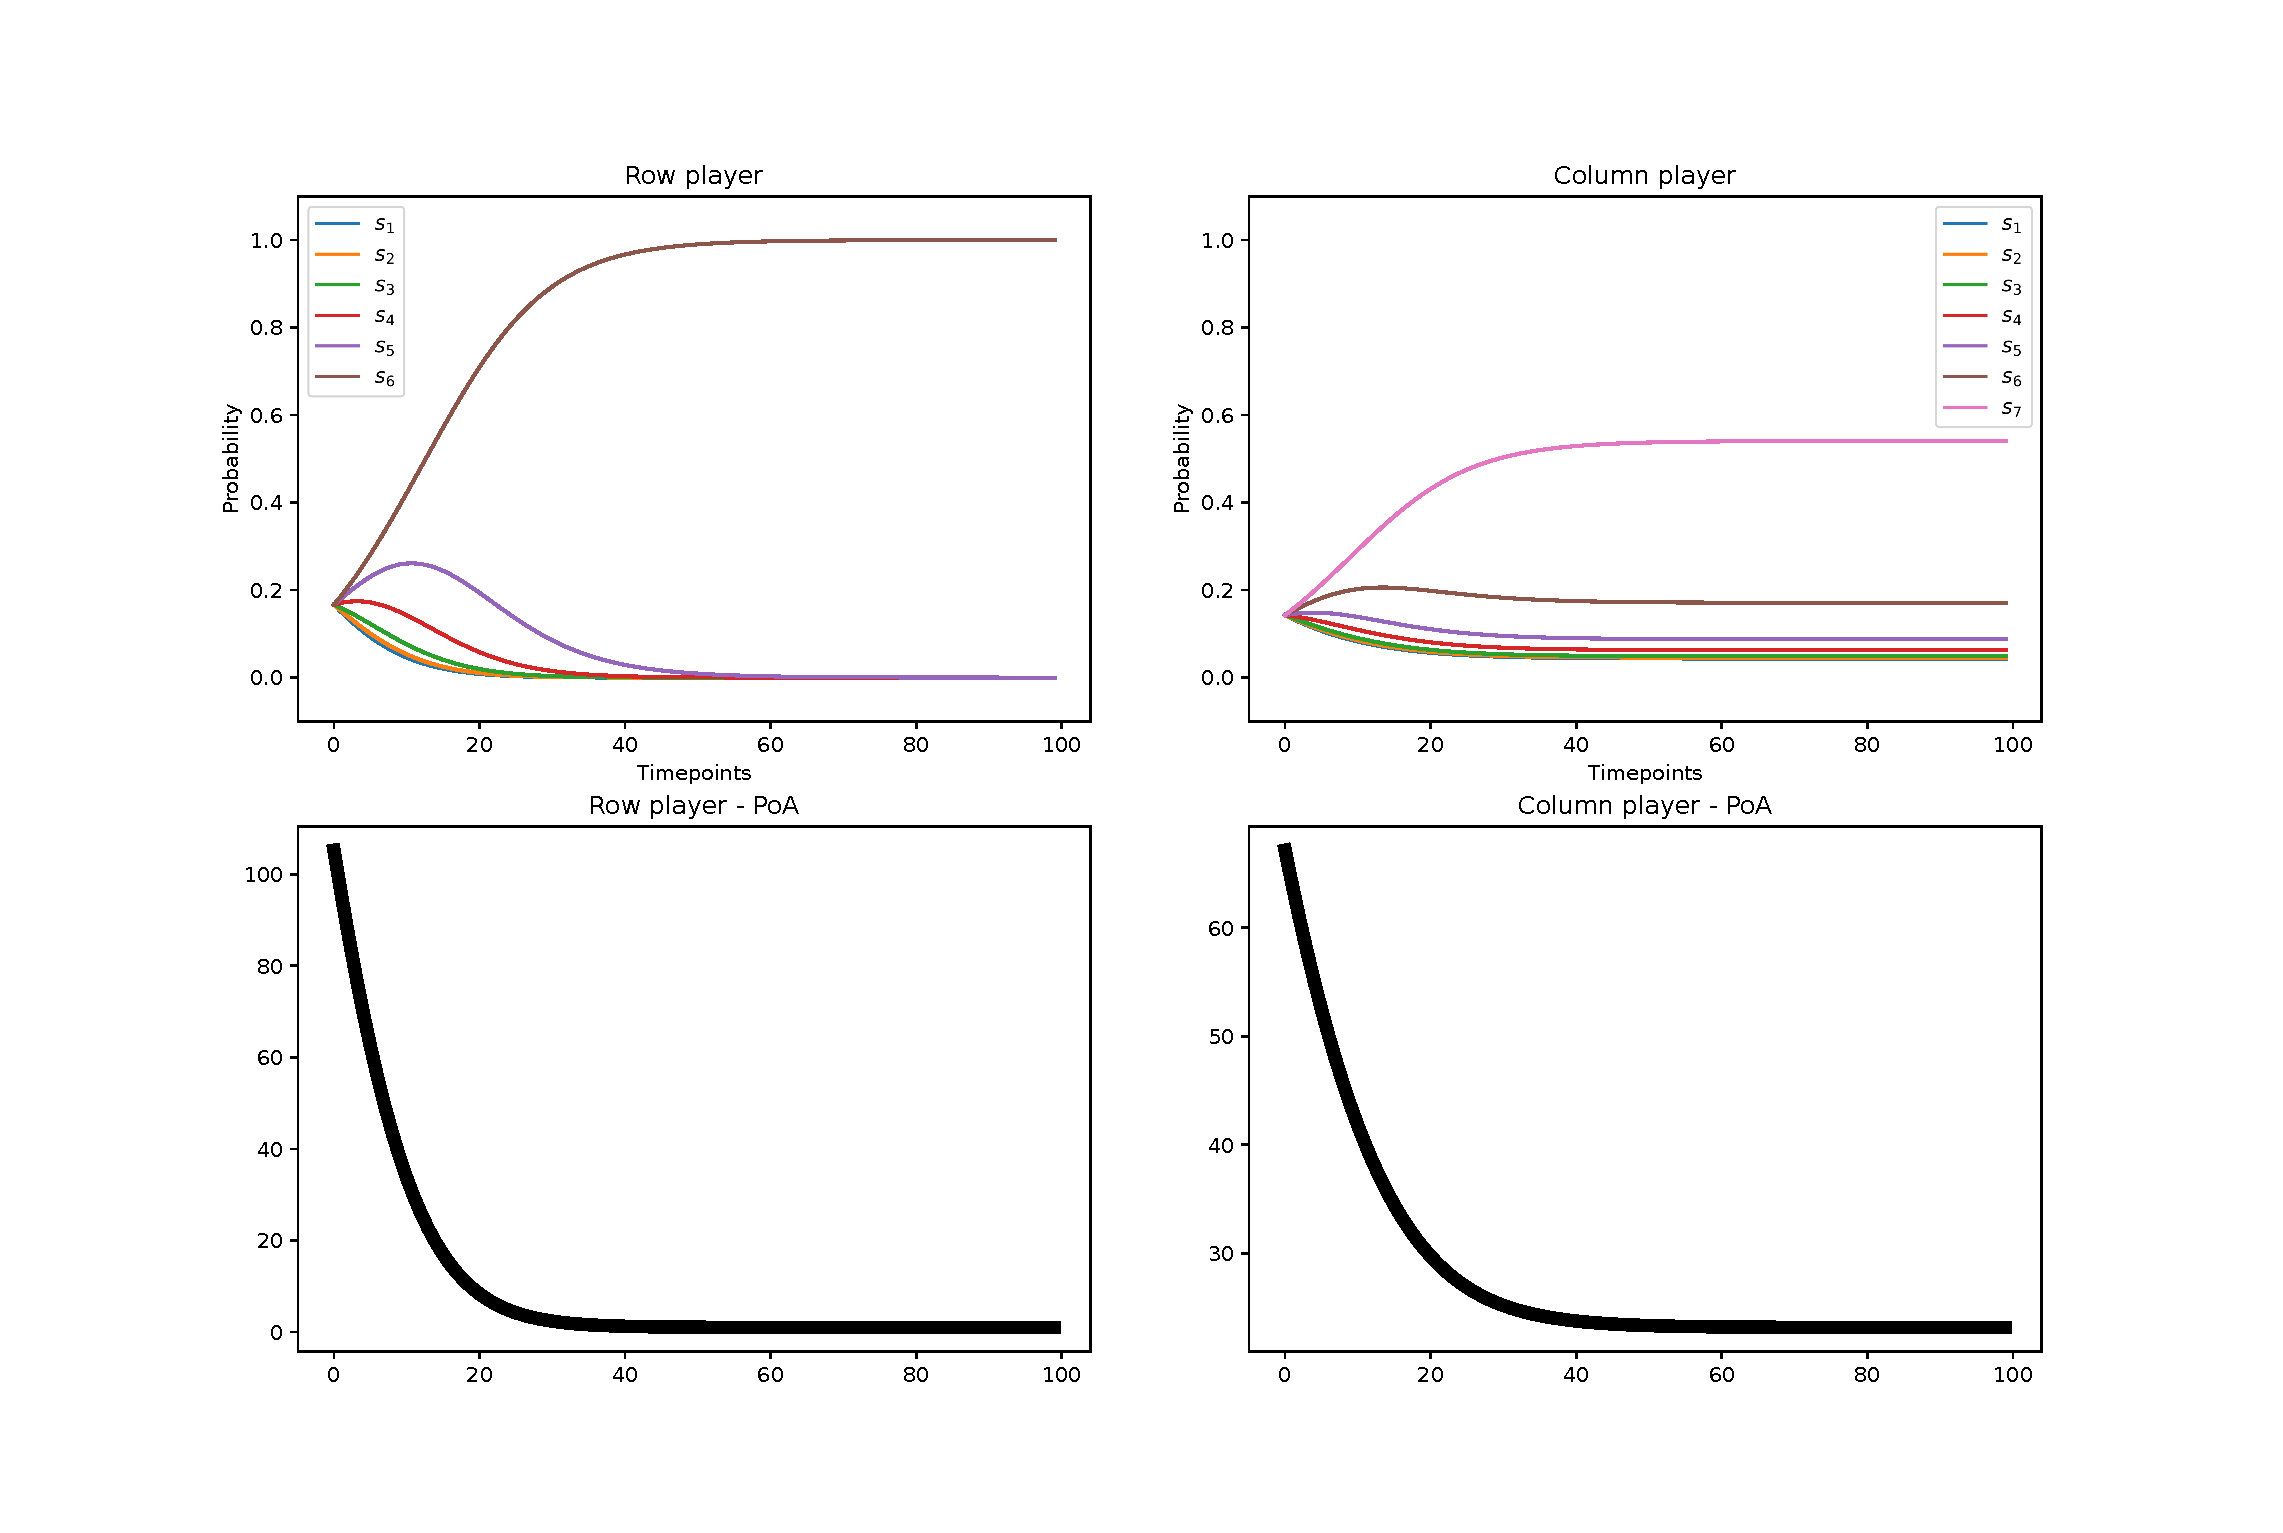
\includegraphics[width=\textwidth, trim = 0 60 0 60, clip]{chapters/00_appendix/02_more_game_results/Bin/poa_ard_target_3.eps}
    \caption{Asymmetric replicator dynamics run and PoA of the game theoretic
    model with time target 3.0 and parameters: \(\alpha = 0.97,
    \lambda_2 = 0.1, \lambda_1^{(1)} = 3.0, \lambda_1^{(2)} = 4.5,
    \mu^{(1)} = 2.0, \mu^{(2)} = 3.0, C^{(1)} = 3, C^{(2)} = 2,
    N^{(1)} = 6, N^{(2)} = 7, M^{(1)} = 5, M^{(2)} = 4\).}
    \label{fig:poa_ard_target_3}
\end{figure}

\begin{figure}[H]
    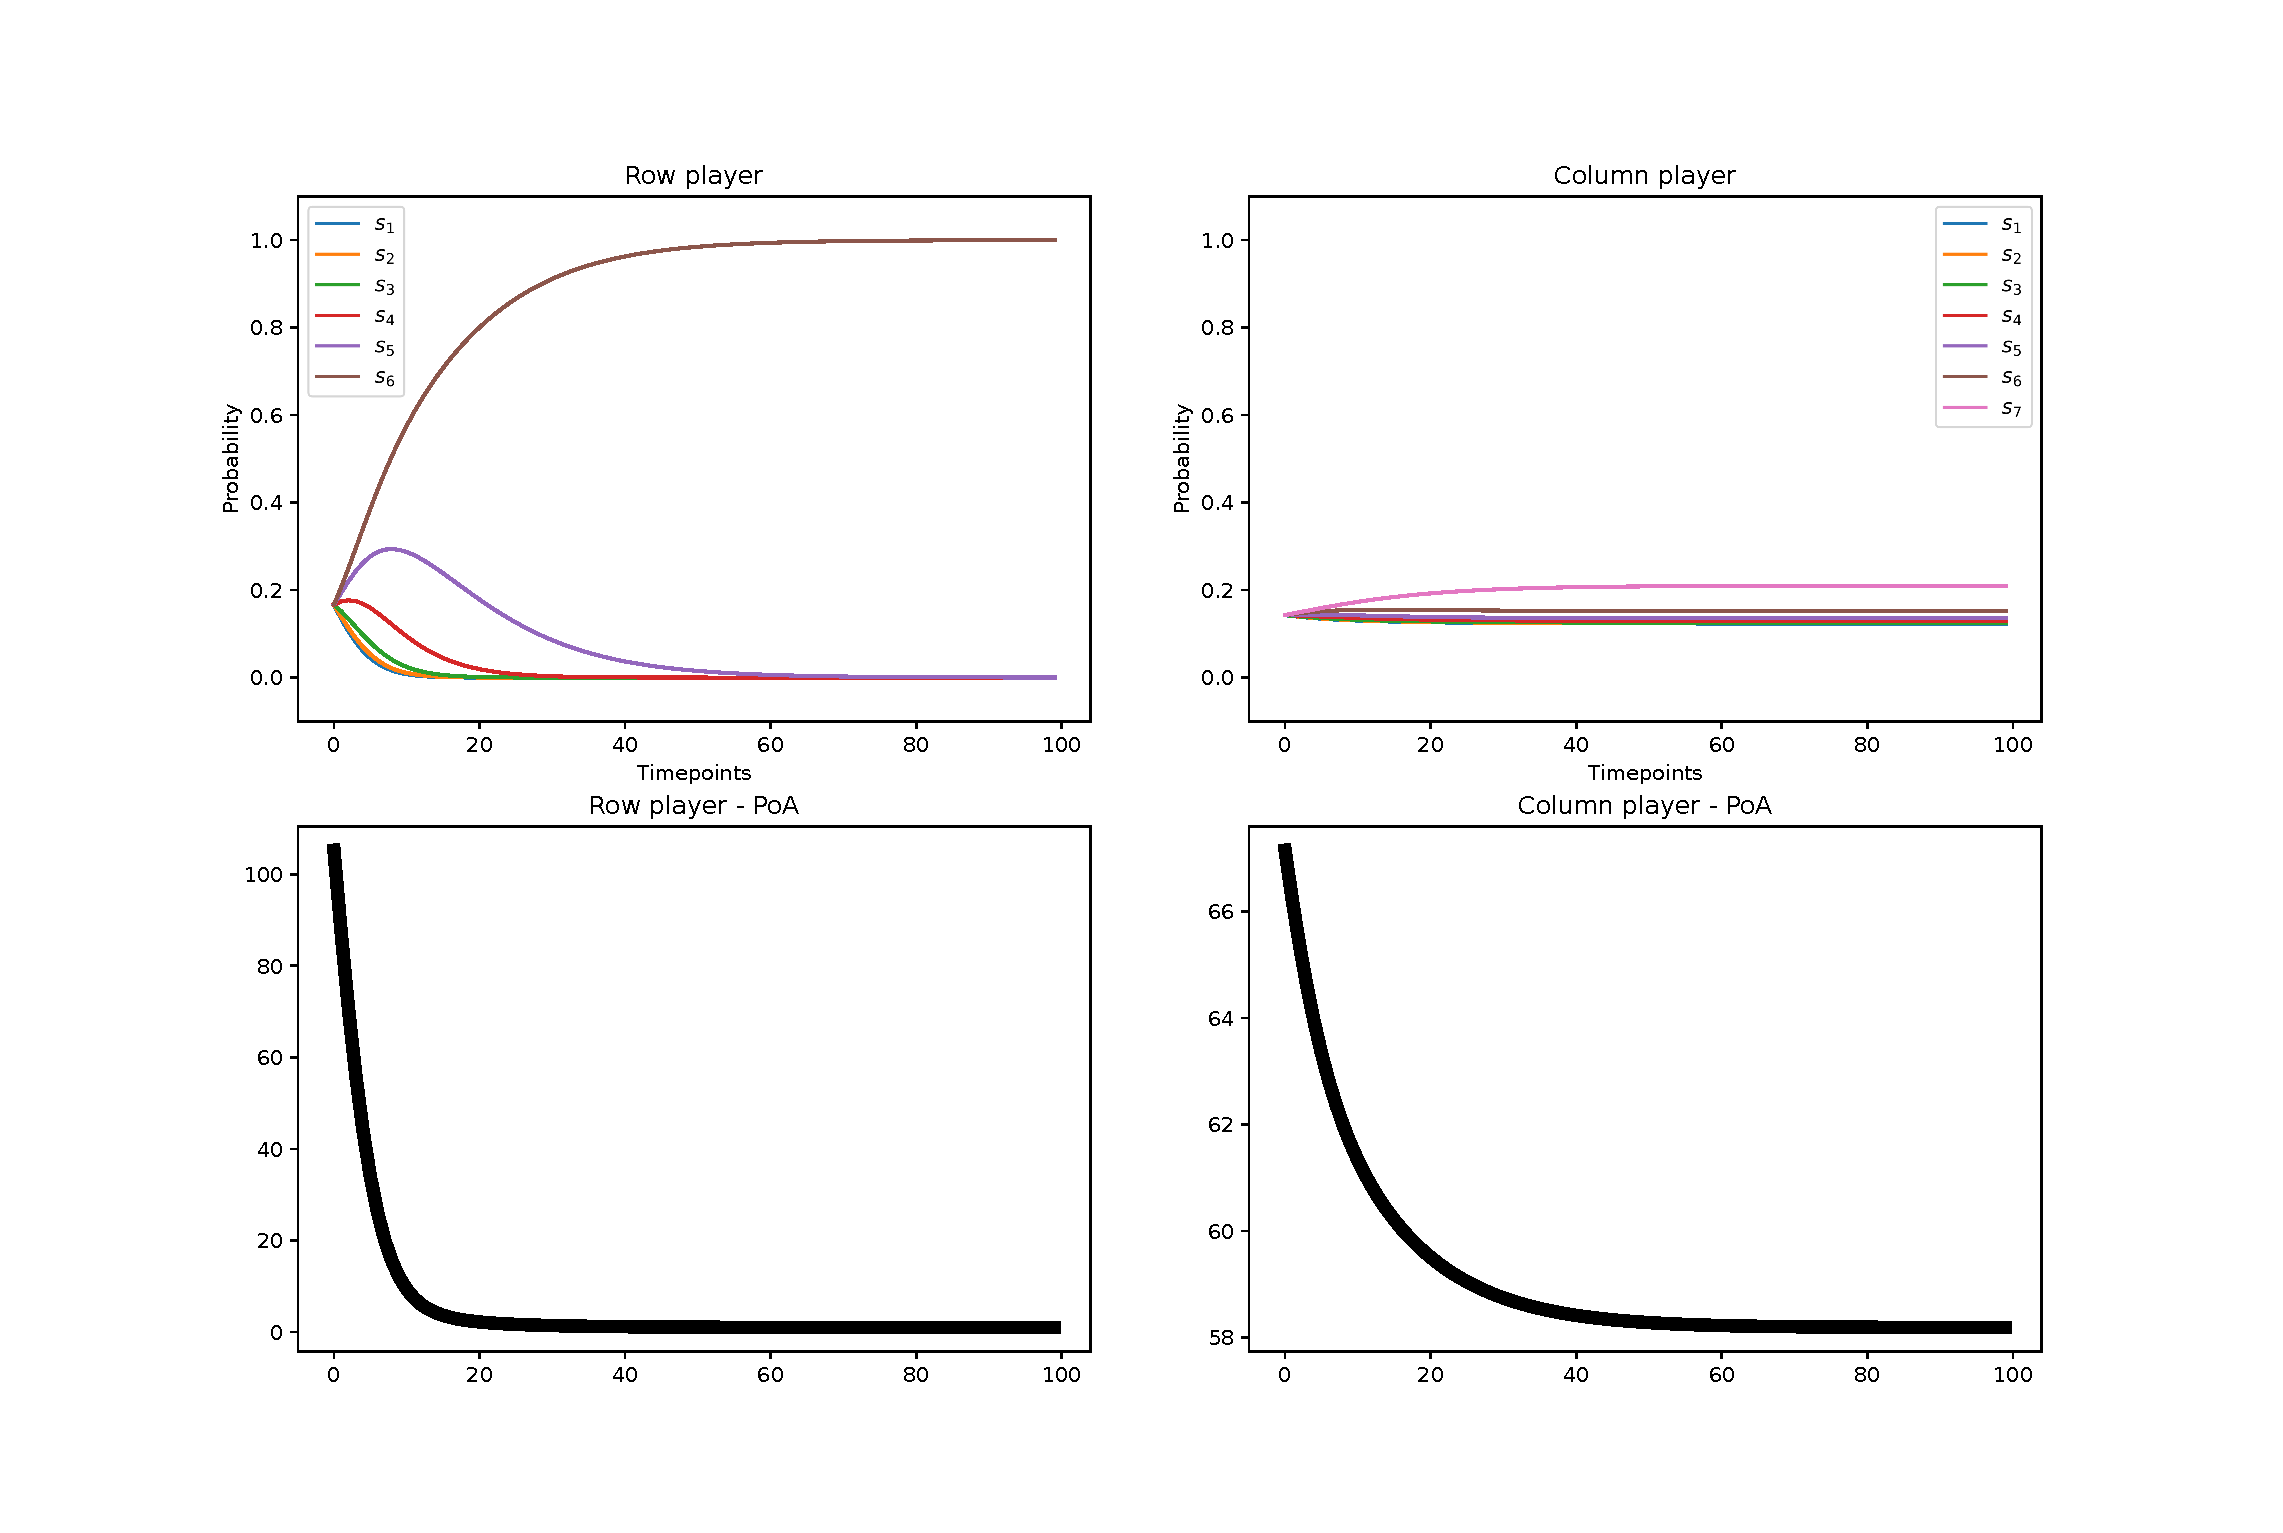
\includegraphics[width=\textwidth, trim = 0 60 0 60, clip]{chapters/00_appendix/02_more_game_results/Bin/poa_ard_target_5.eps}
    \caption{Asymmetric replicator dynamics run and PoA of the game theoretic
    model with time target 5.0 and parameters: \(\alpha = 0.97,
    \lambda_2 = 0.1, \lambda_1^{(1)} = 3.0, \lambda_1^{(2)} = 4.5,
    \mu^{(1)} = 2.0, \mu^{(2)} = 3.0, C^{(1)} = 3, C^{(2)} = 2,
    N^{(1)} = 6, N^{(2)} = 7, M^{(1)} = 5, M^{(2)} = 4\).}
    \label{fig:poa_ard_target_5}
\end{figure}


\begin{figure}[H]
    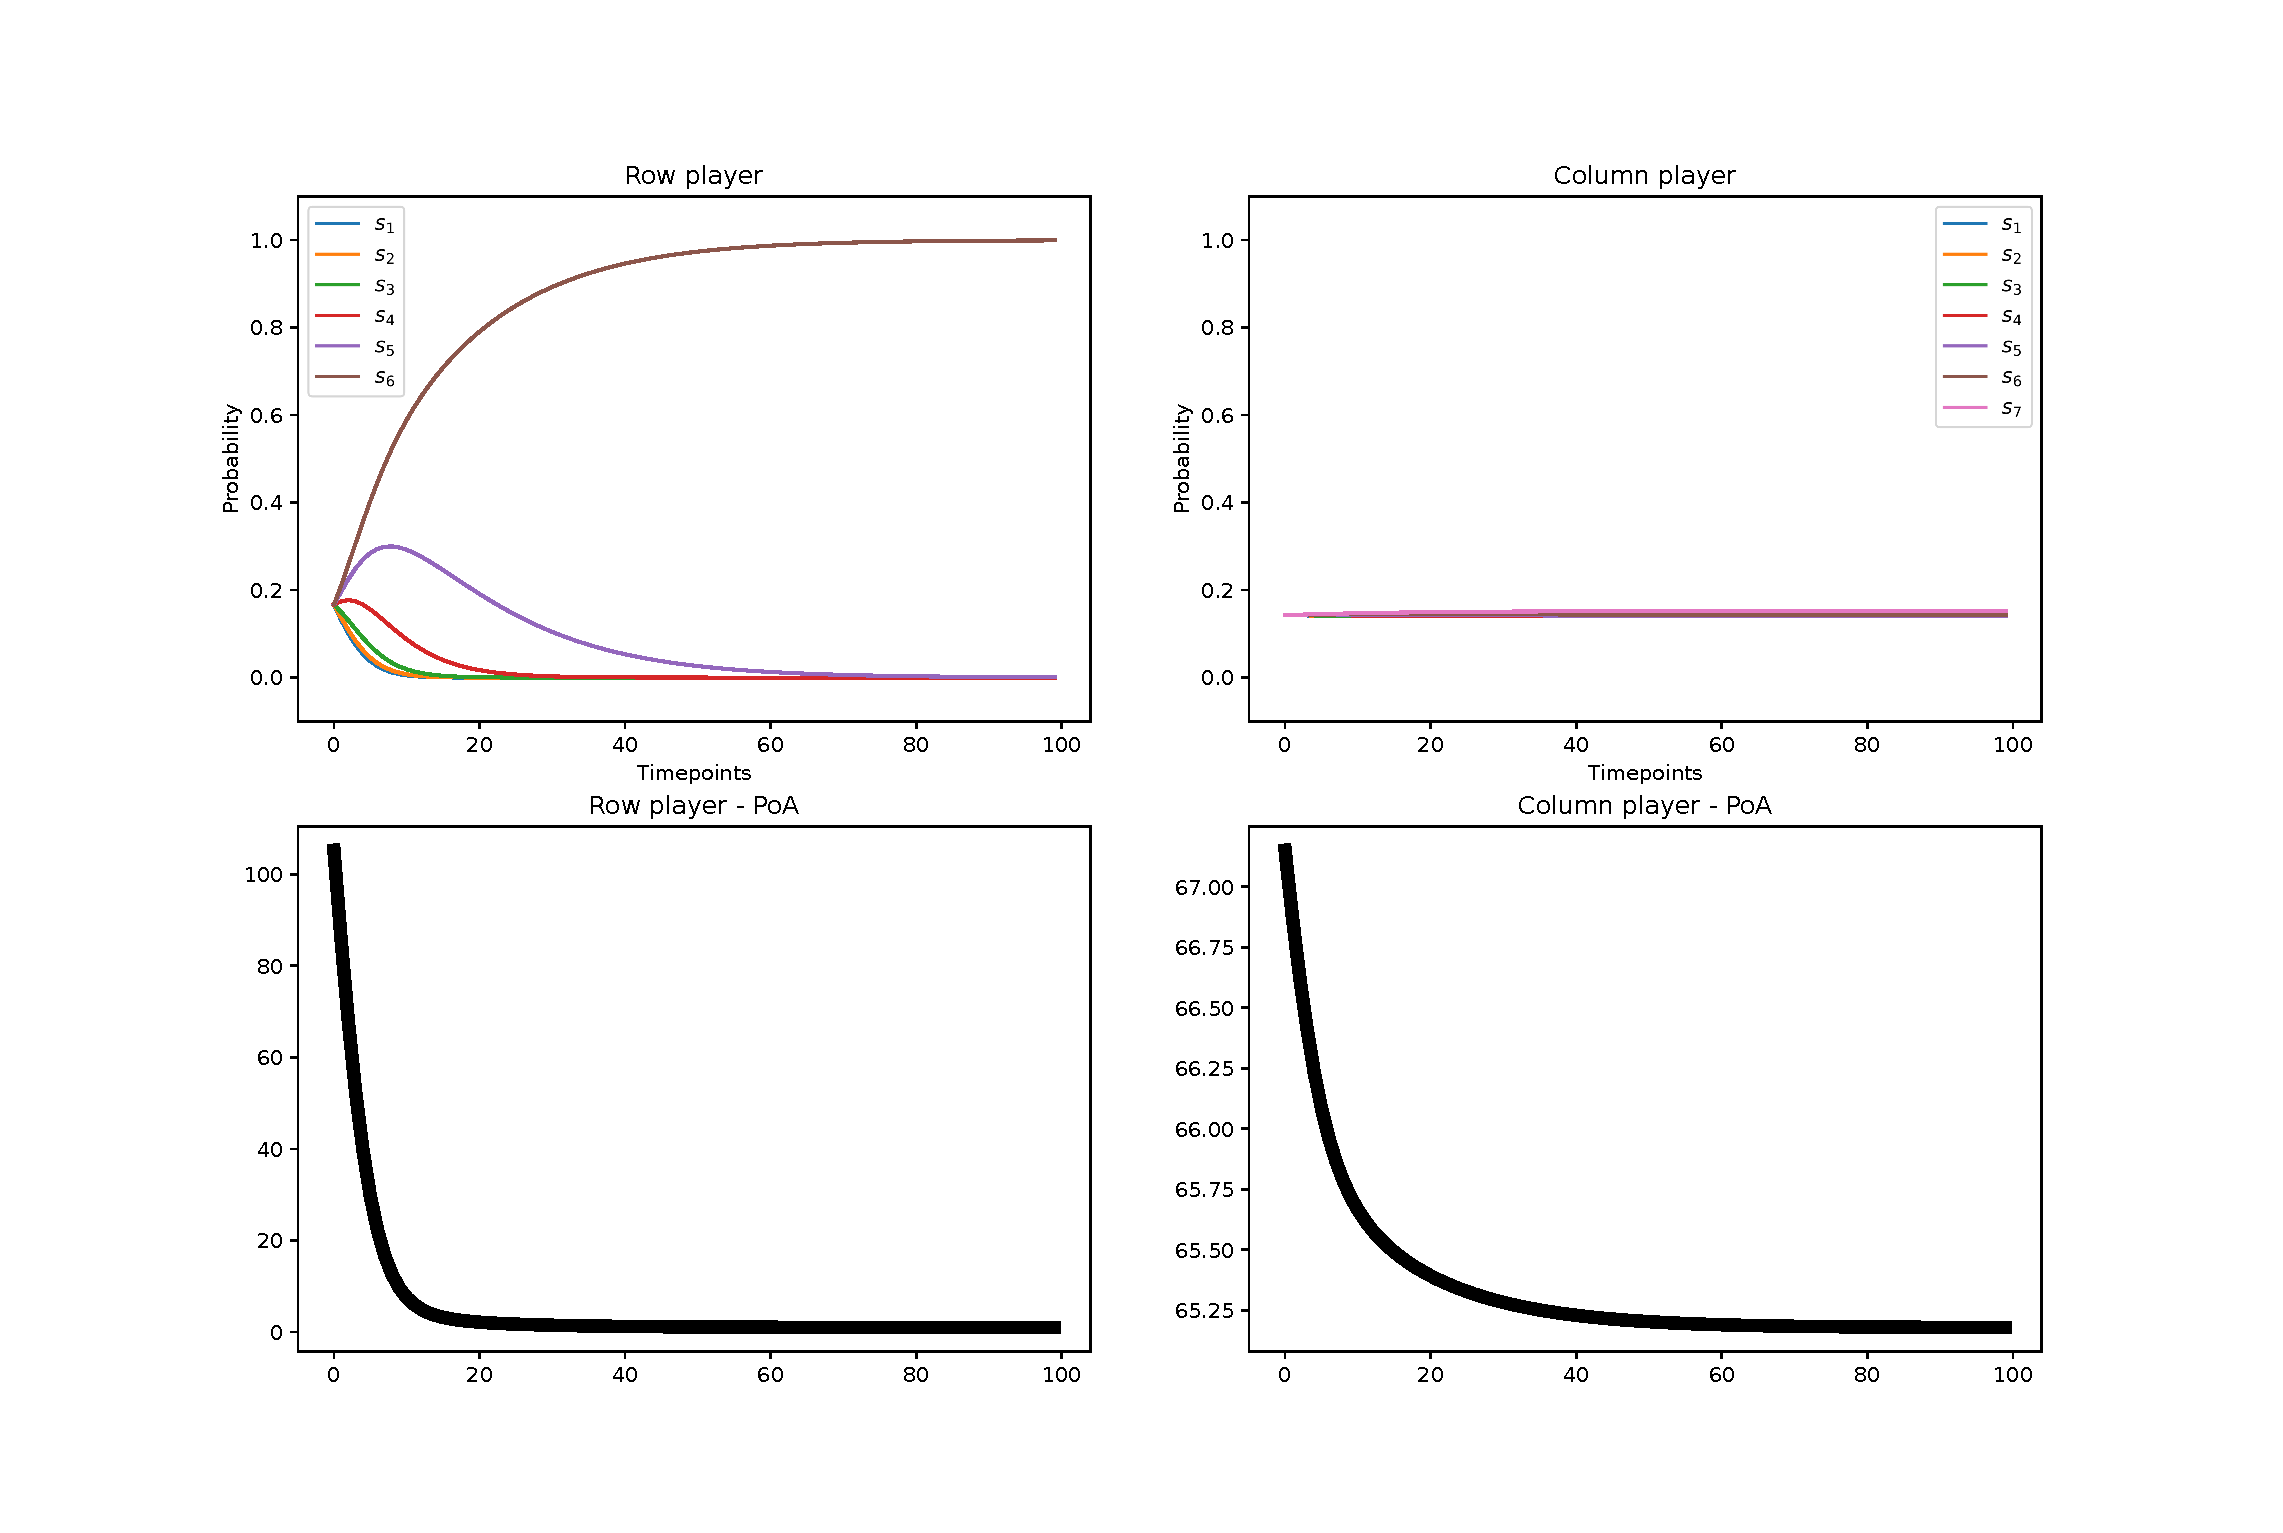
\includegraphics[width=\textwidth, trim = 0 60 0 60, clip]{chapters/00_appendix/02_more_game_results/Bin/poa_ard_target_7.eps}
    \caption{Asymmetric replicator dynamics run and PoA of the game theoretic
    model with time target 7.0 and parameters: \(\alpha = 0.97,
    \lambda_2 = 0.1, \lambda_1^{(1)} = 3.0, \lambda_1^{(2)} = 4.5,
    \mu^{(1)} = 2.0, \mu^{(2)} = 3.0, C^{(1)} = 3, C^{(2)} = 2,
    N^{(1)} = 6, N^{(2)} = 7, M^{(1)} = 5, M^{(2)} = 4\).}
    \label{fig:poa_ard_target_7}
\end{figure}

\begin{figure}[H]
    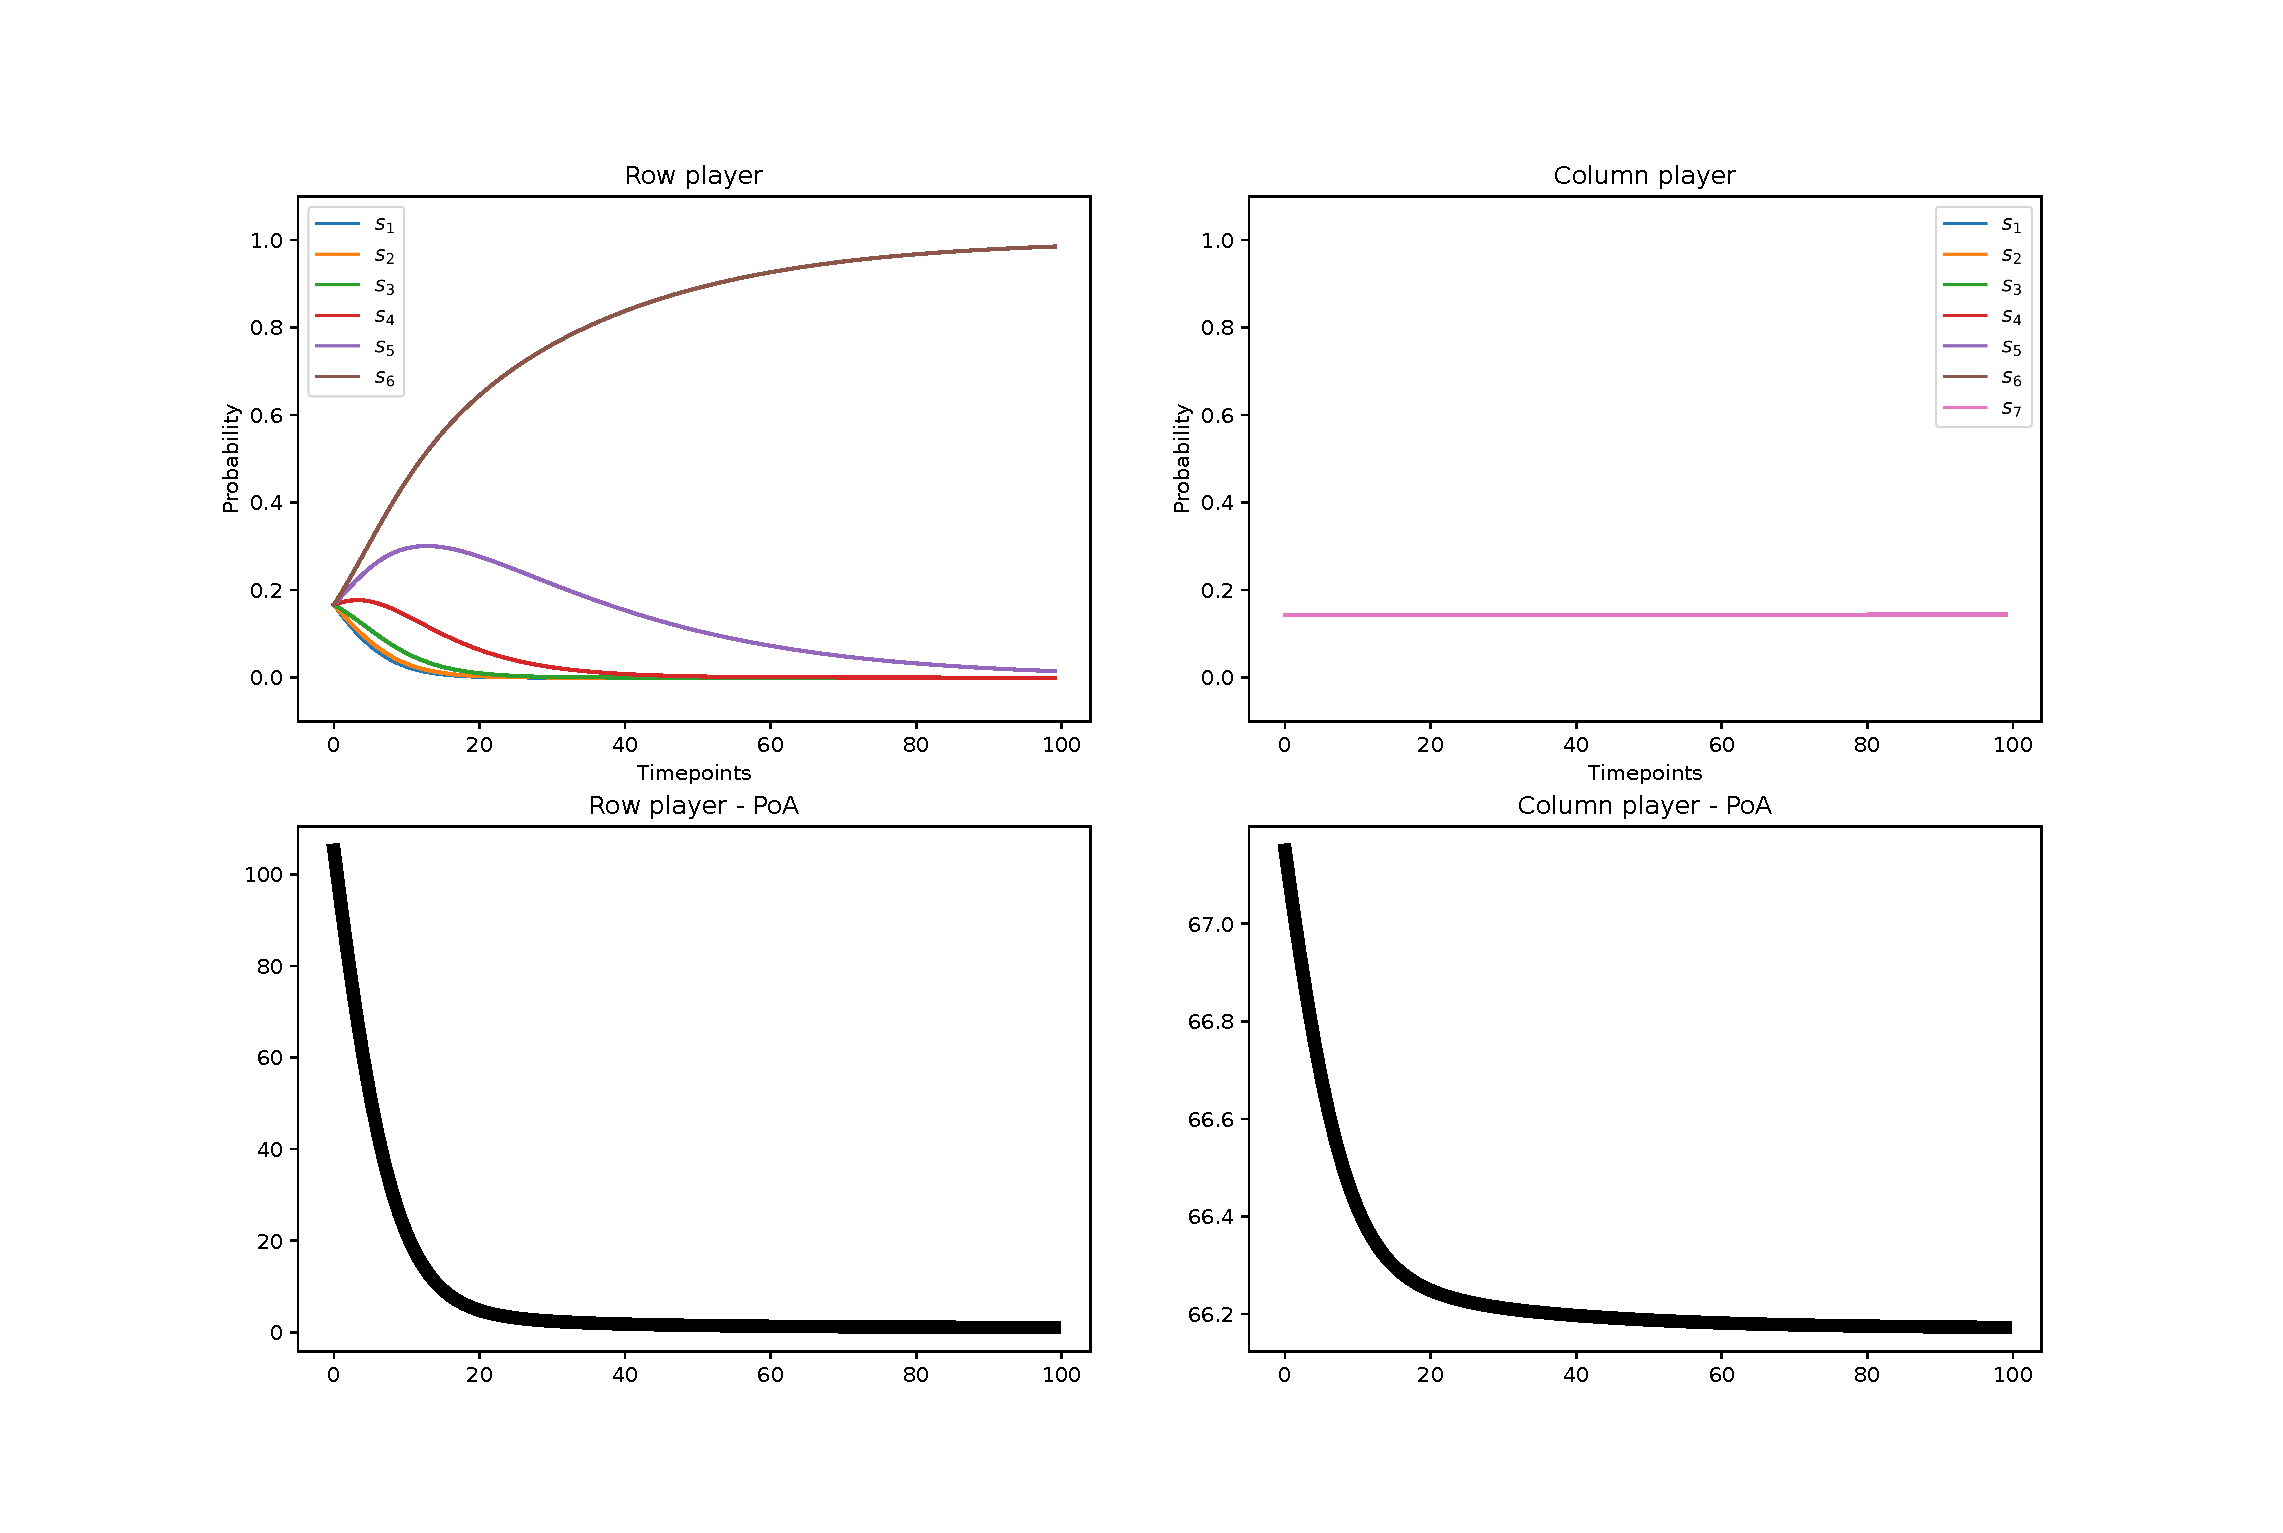
\includegraphics[width=\textwidth, trim = 0 60 0 60, clip]{chapters/00_appendix/02_more_game_results/Bin/poa_ard_target_9.eps}
    \caption{Asymmetric replicator dynamics run and PoA of the game theoretic
    model with time target 9.0 and parameters: \(\alpha = 0.97,
    \lambda_2 = 0.1, \lambda_1^{(1)} = 3.0, \lambda_1^{(2)} = 4.5,
    \mu^{(1)} = 2.0, \mu^{(2)} = 3.0, C^{(1)} = 3, C^{(2)} = 2,
    N^{(1)} = 6, N^{(2)} = 7, M^{(1)} = 5, M^{(2)} = 4\).}
    \label{fig:poa_ard_target_9}
\end{figure}


\section{Multiple values of ``weight'' parameter}\label{app:b_2}


\begin{figure}[H]
    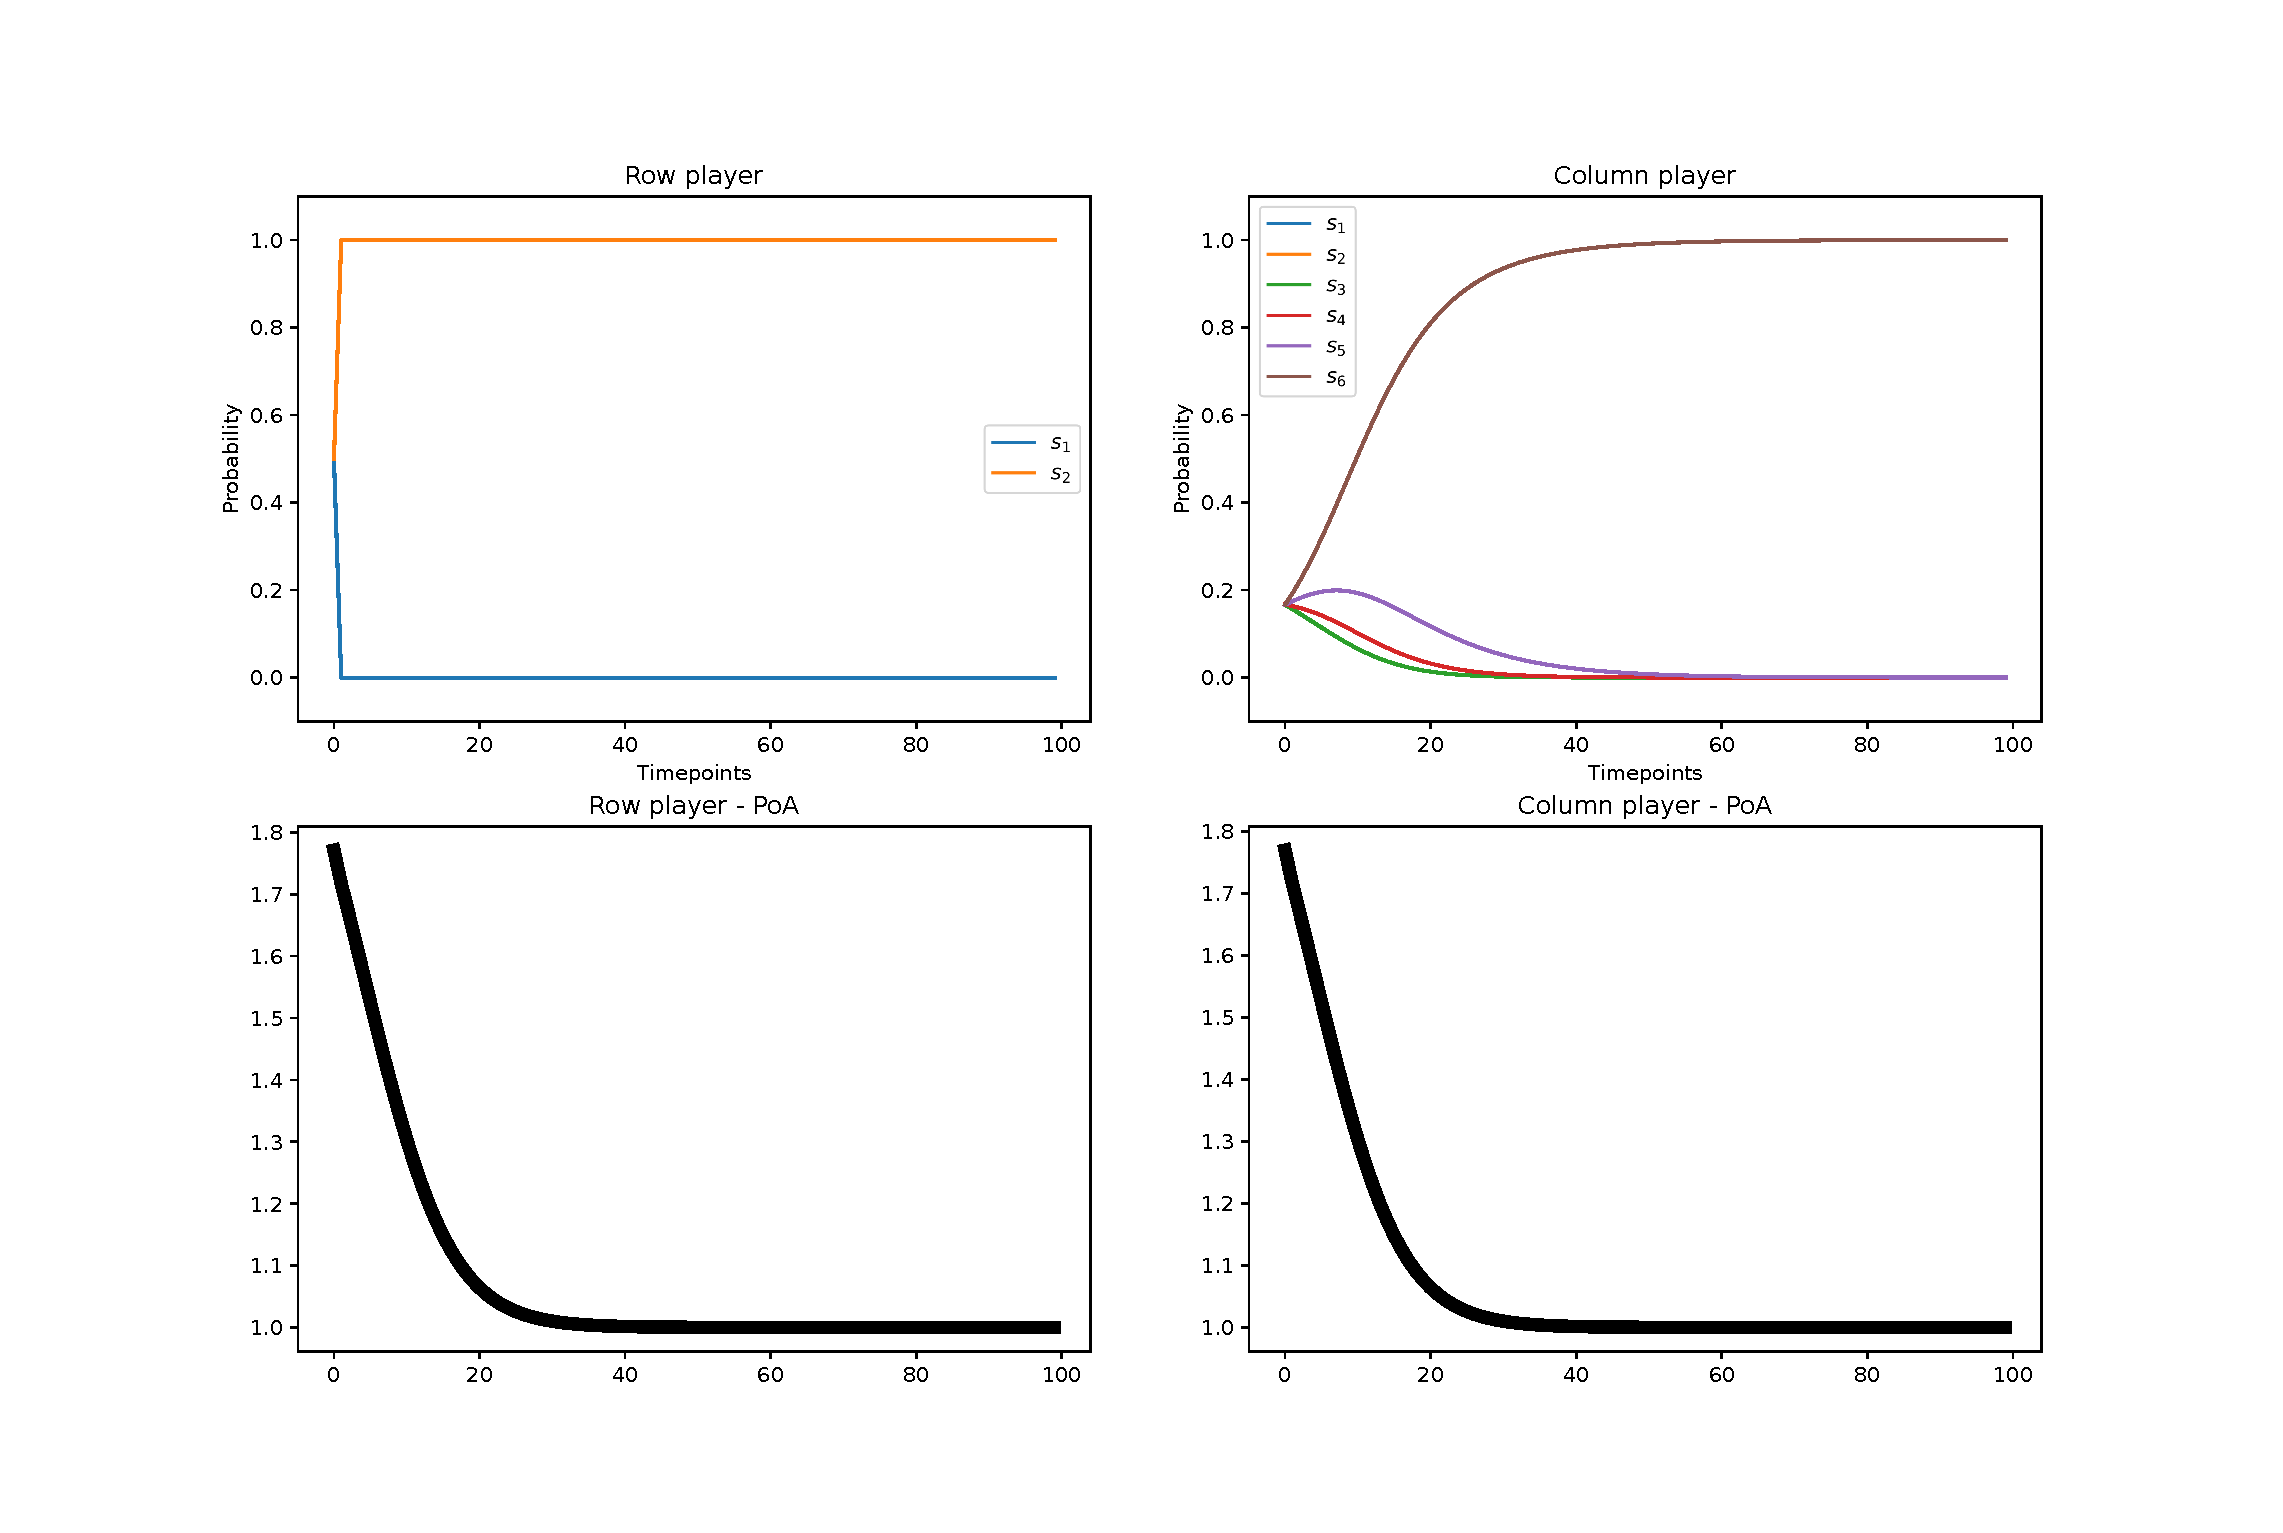
\includegraphics[width=\textwidth, trim = 0 60 0 60, clip]{chapters/00_appendix/02_more_game_results/Bin/poa_ard_alpha_0.eps}
    \caption{Asymmetric replicator dynamics run and PoA of the game theoretic
    model with \(\alpha = 0.0\) and parameters: \(\lambda_2 = 32.05,
    \lambda_1^{(1)} = 0.0, \lambda_1^{(2)} = 0.0, \mu^{(1)} = 4.2,
    \mu^{(2)} = 6.6, C^{(1)} = 1, C^{(2)} = 3, N^{(1)} = 2, N^{(2)} = 6,
    M^{(1)} = 7, M^{(2)} = 4, t = 2.0\).}
    \label{fig:poa_ard_alpha_0}
\end{figure}



\begin{figure}[H]
    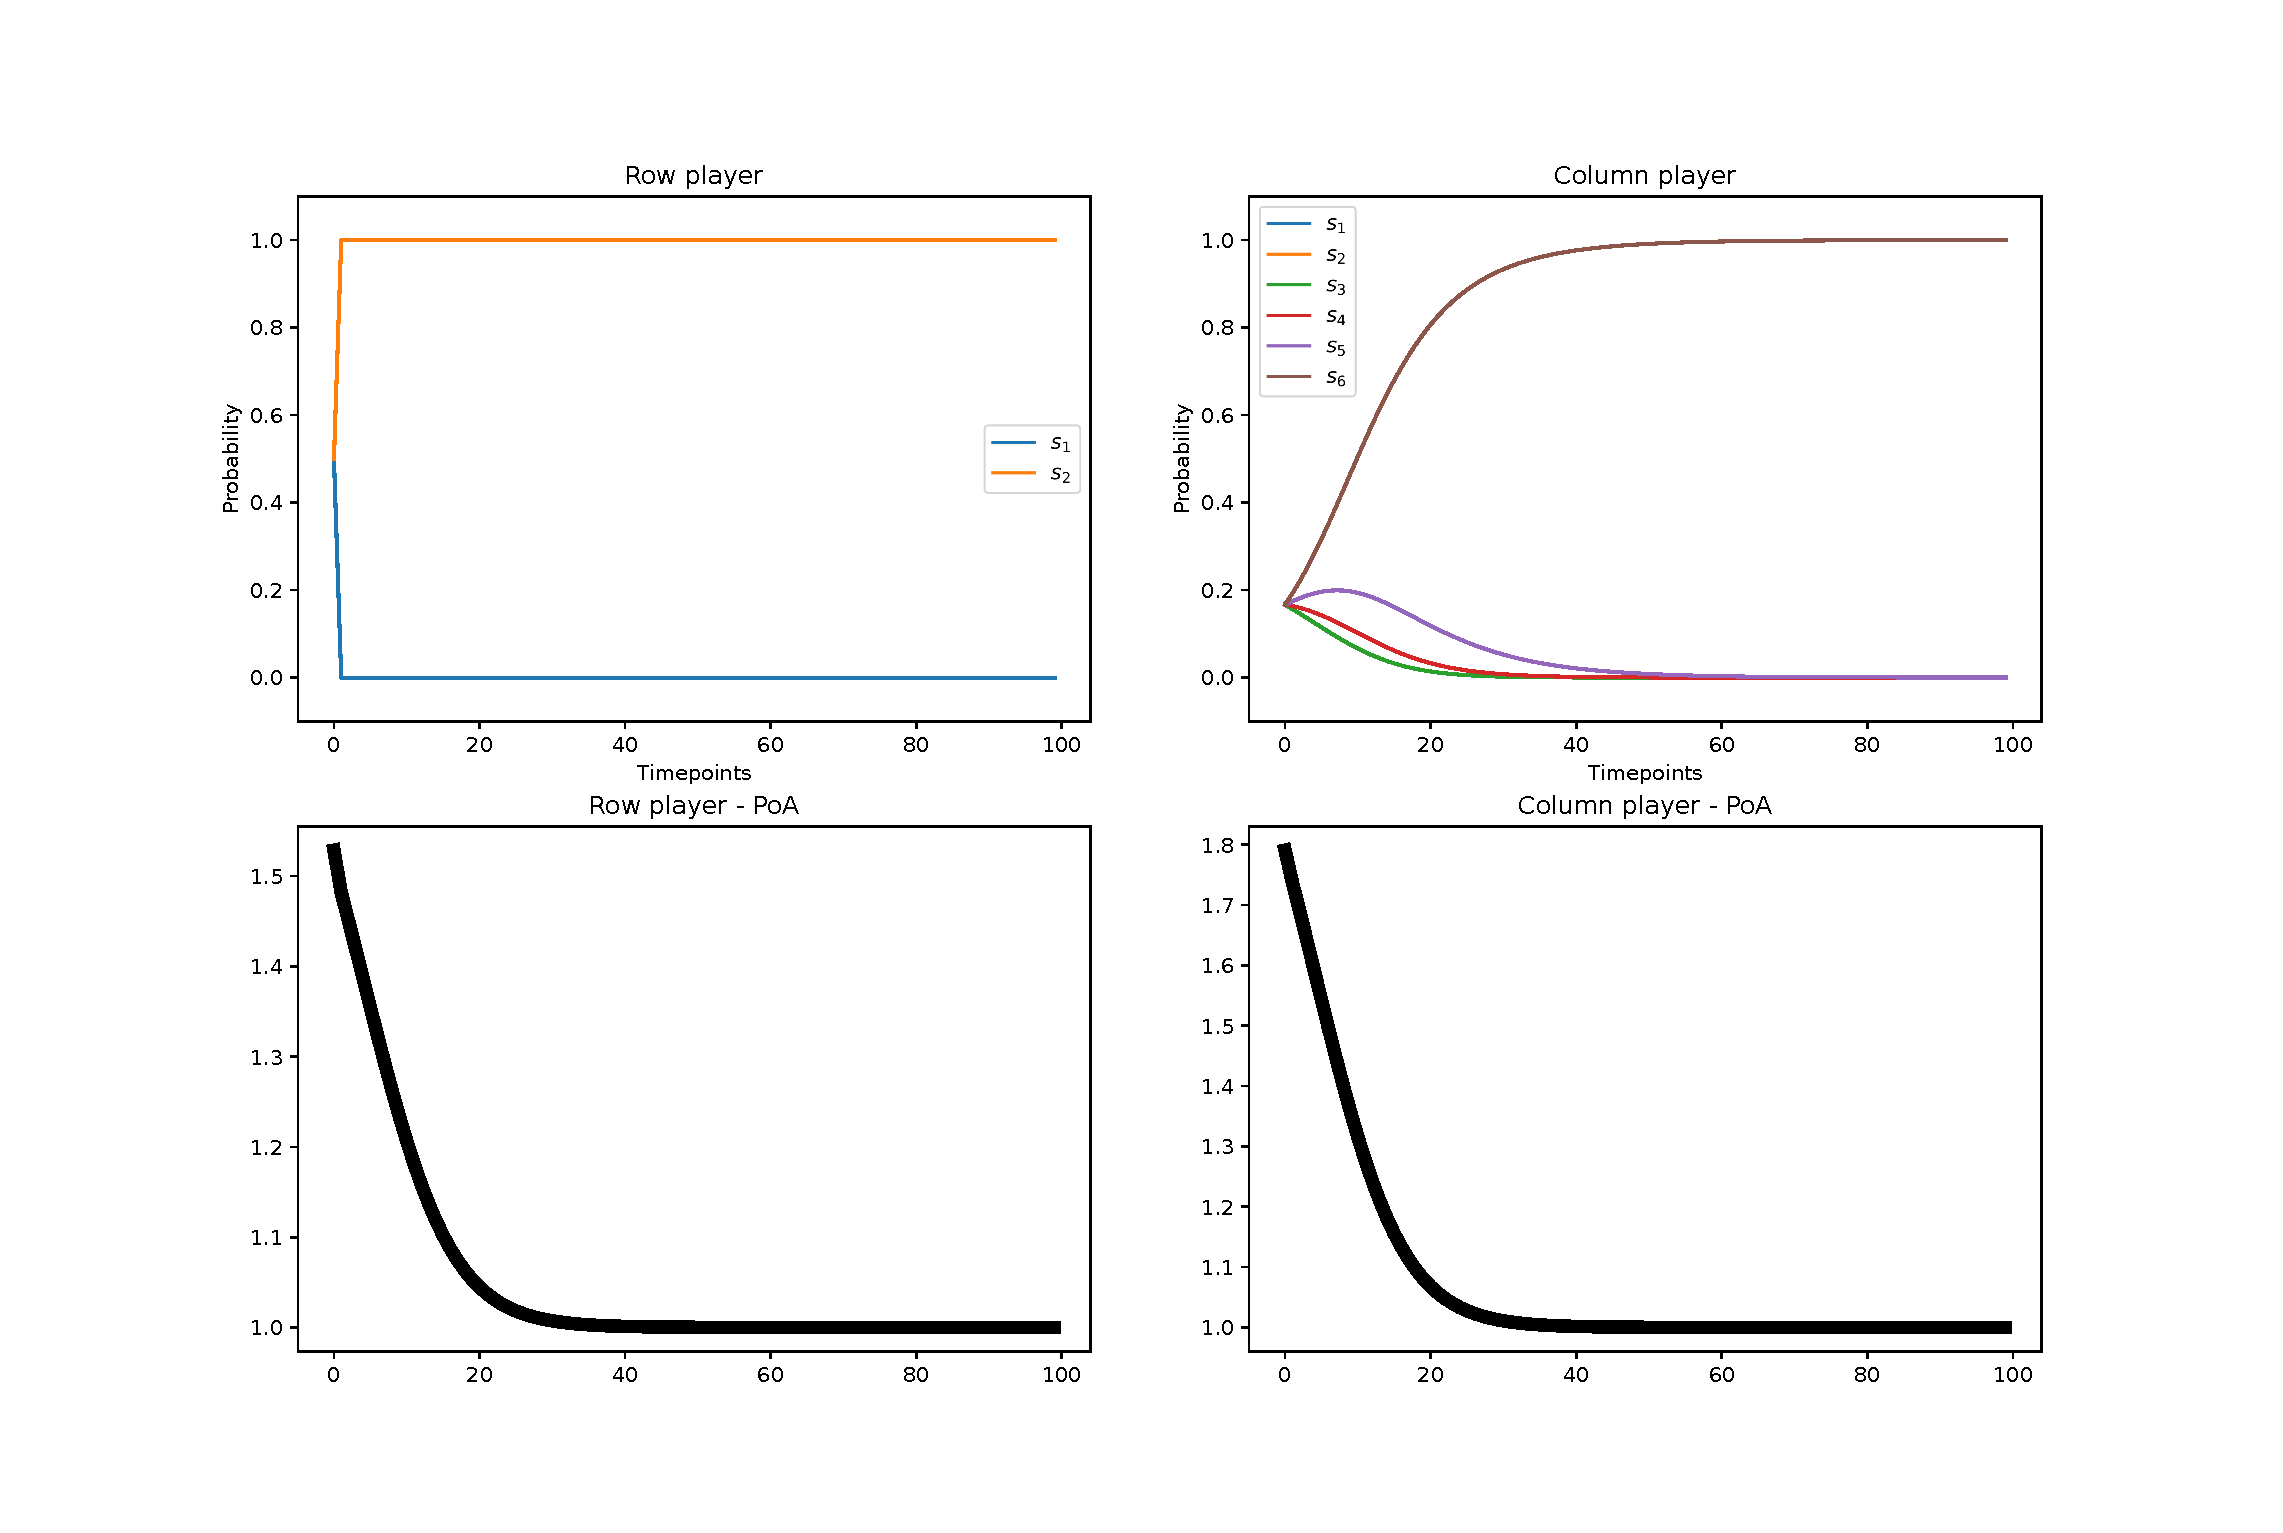
\includegraphics[width=\textwidth, trim = 0 60 0 60, clip]{chapters/00_appendix/02_more_game_results/Bin/poa_ard_alpha_03.eps}
    \caption{Asymmetric replicator dynamics run and PoA of the game theoretic
    model with \(\alpha = 0.3\) and parameters: \(\lambda_2 = 32.05,
    \lambda_1^{(1)} = 0.0, \lambda_1^{(2)} = 0.0, \mu^{(1)} = 4.2,
    \mu^{(2)} = 6.6, C^{(1)} = 1, C^{(2)} = 3, N^{(1)} = 2, N^{(2)} = 6,
    M^{(1)} = 7, M^{(2)} = 4, t = 2.0\).}
    \label{fig:poa_ard_alpha_03}
\end{figure}




\begin{figure}[H]
    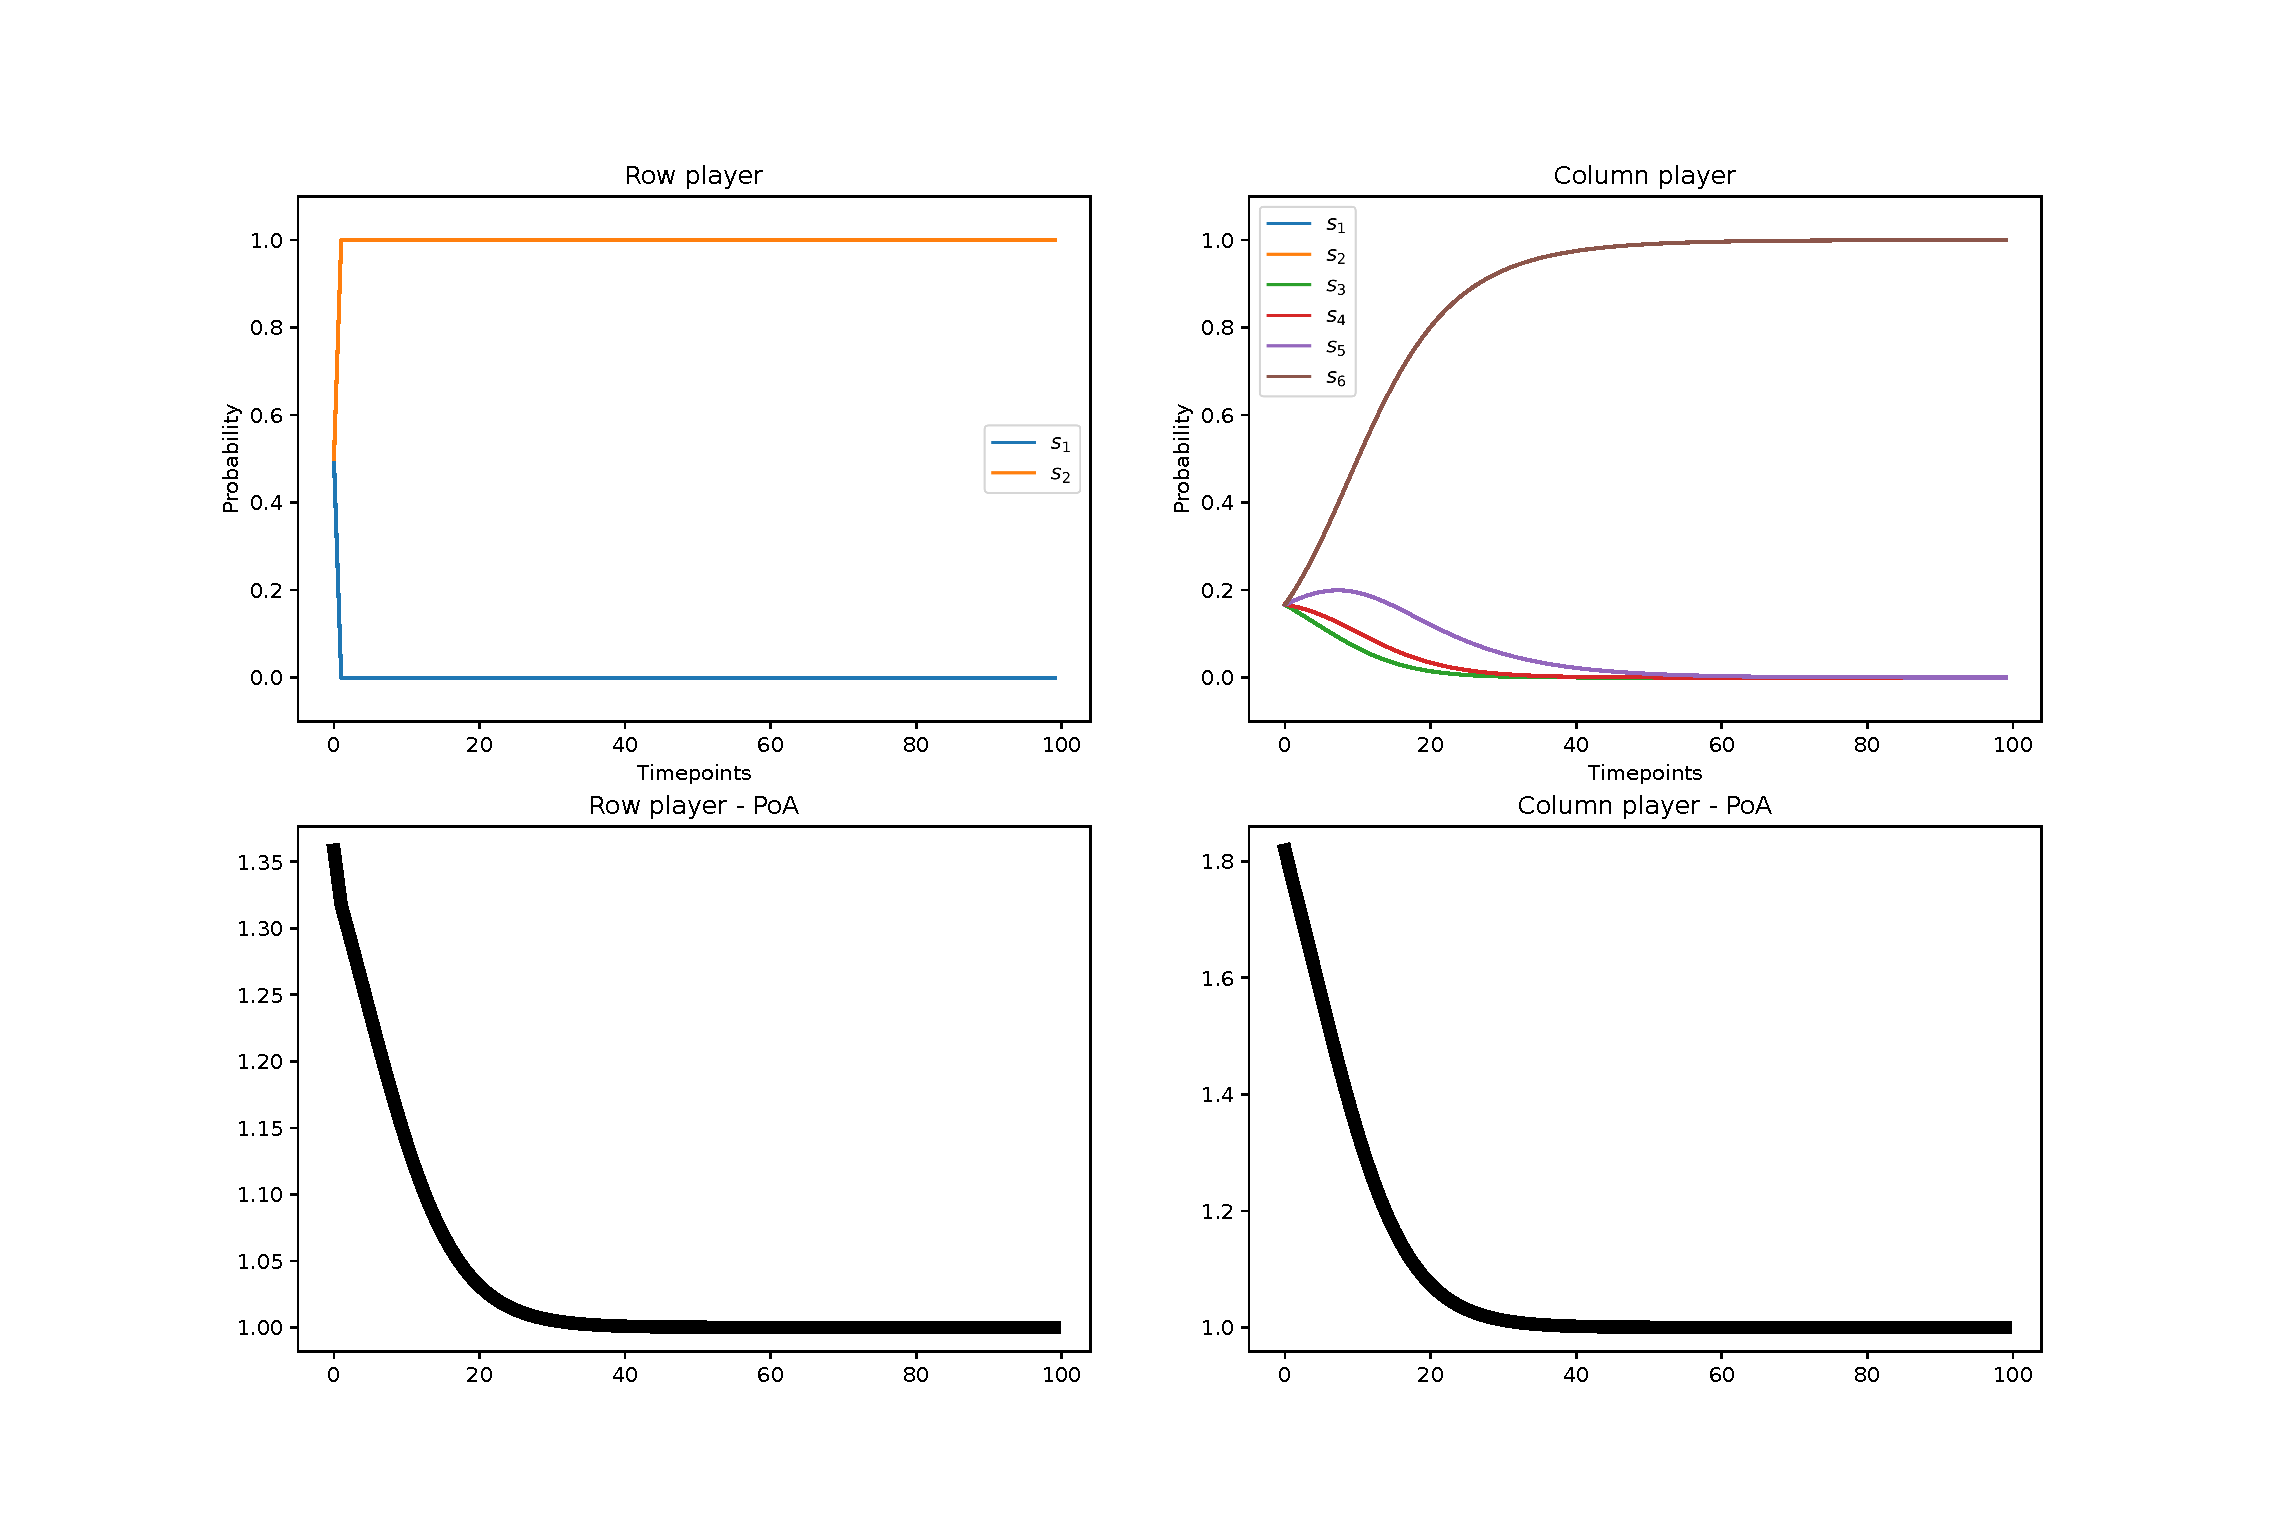
\includegraphics[width=\textwidth, trim = 0 60 0 60, clip]{chapters/00_appendix/02_more_game_results/Bin/poa_ard_alpha_06.eps}
    \caption{Asymmetric replicator dynamics run and PoA of the game theoretic
    model with \(\alpha = 0.6\) and parameters: \(\lambda_2 = 32.05,
    \lambda_1^{(1)} = 0.0, \lambda_1^{(2)} = 0.0, \mu^{(1)} = 4.2,
    \mu^{(2)} = 6.6, C^{(1)} = 1, C^{(2)} = 3, N^{(1)} = 2, N^{(2)} = 6,
    M^{(1)} = 7, M^{(2)} = 4, t = 2.0\).}
    \label{fig:poa_ard_alpha_06}
\end{figure}



\begin{figure}[H]
    \includegraphics[width=\textwidth, trim = 0 60 0 60, clip]{chapters/00_appendix/02_more_game_results/Bin/poa_ard_alpha_09.eps}
    \caption{Asymmetric replicator dynamics run and PoA of the game theoretic
    model with \(\alpha = 0.9\) and parameters: \(\lambda_2 = 32.05,
    \lambda_1^{(1)} = 0.0, \lambda_1^{(2)} = 0.0, \mu^{(1)} = 4.2,
    \mu^{(2)} = 6.6, C^{(1)} = 1, C^{(2)} = 3, N^{(1)} = 2, N^{(2)} = 6,
    M^{(1)} = 7, M^{(2)} = 4, t = 2.0\).}
    \label{fig:poa_ard_alpha_09}
\end{figure}



\begin{figure}[H]
    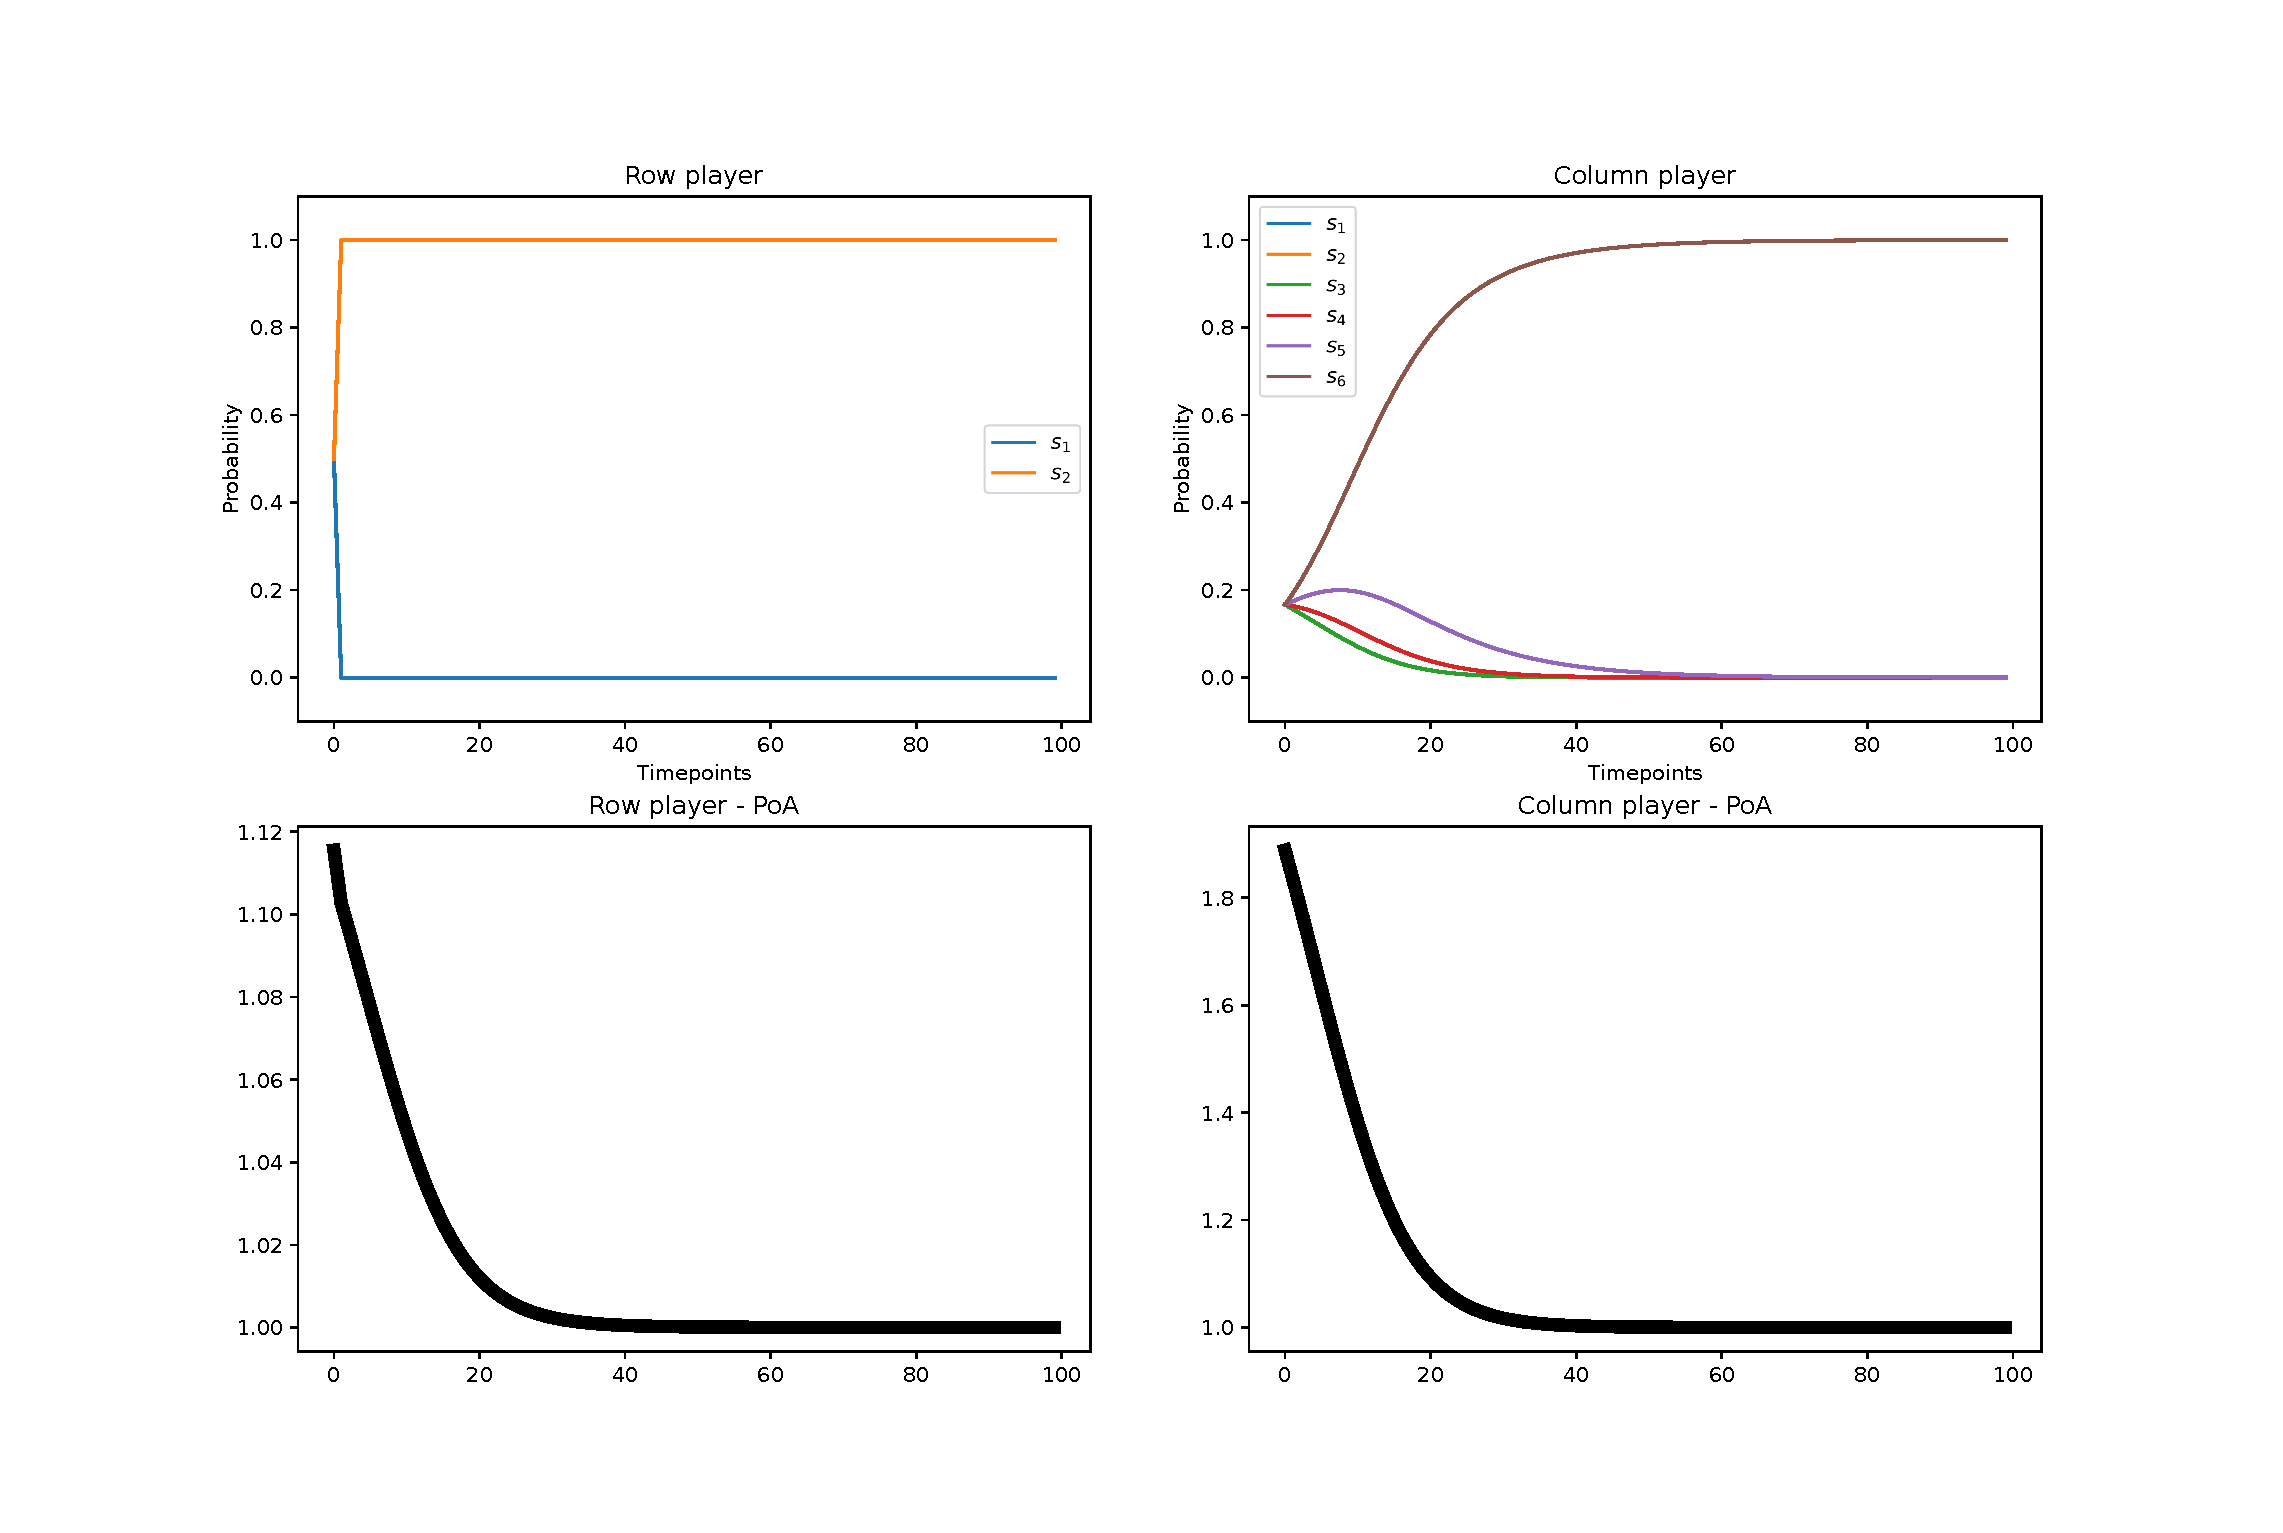
\includegraphics[width=\textwidth, trim = 0 60 0 60, clip]{chapters/00_appendix/02_more_game_results/Bin/poa_ard_alpha_1.eps}
    \caption{Asymmetric replicator dynamics run and PoA of the game theoretic
    model with \(\alpha = 1\) and parameters: \(\lambda_2 = 32.05,
    \lambda_1^{(1)} = 0.0, \lambda_1^{(2)} = 0.0, \mu^{(1)} = 4.2,
    \mu^{(2)} = 6.6, C^{(1)} = 1, C^{(2)} = 3, N^{(1)} = 2, N^{(2)} = 6,
    M^{(1)} = 7, M^{(2)} = 4, t = 2.0\).}
    \label{fig:poa_ard_alpha_1}
\end{figure}


\section{Other numerical results}\label{app:b_3}


\begin{figure}[H]
    \includegraphics[width=\textwidth, trim = 0 60 0 60, clip]{chapters/00_appendix/02_more_game_results/Bin/poa_ard_other_1.eps}
    \caption{Asymmetric replicator dynamics run and PoA of the game theoretic
    model with parameters: \(\alpha = 0.95, \lambda_2 = 36.04, t = 6.0,
    \lambda_1^{(1)} = 15.24, \lambda_1^{(2)} = 0.0, \mu^{(1)} = 6.77,
    \mu^{(2)} = 2.22, C^{(1)} = 9, C^{(2)} = 9, N^{(1)} = 10, N^{(2)} = 9,
    M^{(1)} = 4, M^{(2)} = 3\).}
    \label{fig:poa_ard_other_1}
\end{figure}


\begin{figure}[H]
    \includegraphics[width=\textwidth, trim = 0 60 0 60, clip]{chapters/00_appendix/02_more_game_results/Bin/poa_ard_other_2.eps}
    \caption{Asymmetric replicator dynamics run and PoA of the game theoretic
    model with parameters: \(\alpha = 0.96, \lambda_2 = 21.4, t = 1.0,
    \lambda_1^{(1)} = 4.2, \lambda_1^{(2)} = 19.8, \mu^{(1)} = 4.2,
    \mu^{(2)} = 6.6, C^{(1)} = 1, C^{(2)} = 3, N^{(1)} = 2, N^{(2)} = 6,
    M^{(1)} = 7, M^{(2)} = 4\).}
    \label{fig:poa_ard_other_2}
\end{figure}


\begin{figure}[H]
    \includegraphics[width=\textwidth, trim = 0 60 0 60, clip]{chapters/00_appendix/02_more_game_results/Bin/poa_ard_other_3.eps}
    \caption{Asymmetric replicator dynamics run and PoA of the game theoretic
    model with parameters: \(\alpha = 0.97, \lambda_2 = 18.7, t = 2.0,
    \lambda_1^{(1)} = 4.5, \lambda_1^{(2)} = 3.0, \mu^{(1)} = 2.0,
    \mu^{(2)} = 3.0, C^{(1)} = 3, C^{(2)} = 2, N^{(1)} = 6, N^{(2)} = 7,
    M^{(1)} = 5, M^{(2)} = 4\).}
    \label{fig:poa_ard_other_3}
\end{figure}



\begin{figure}[H]
    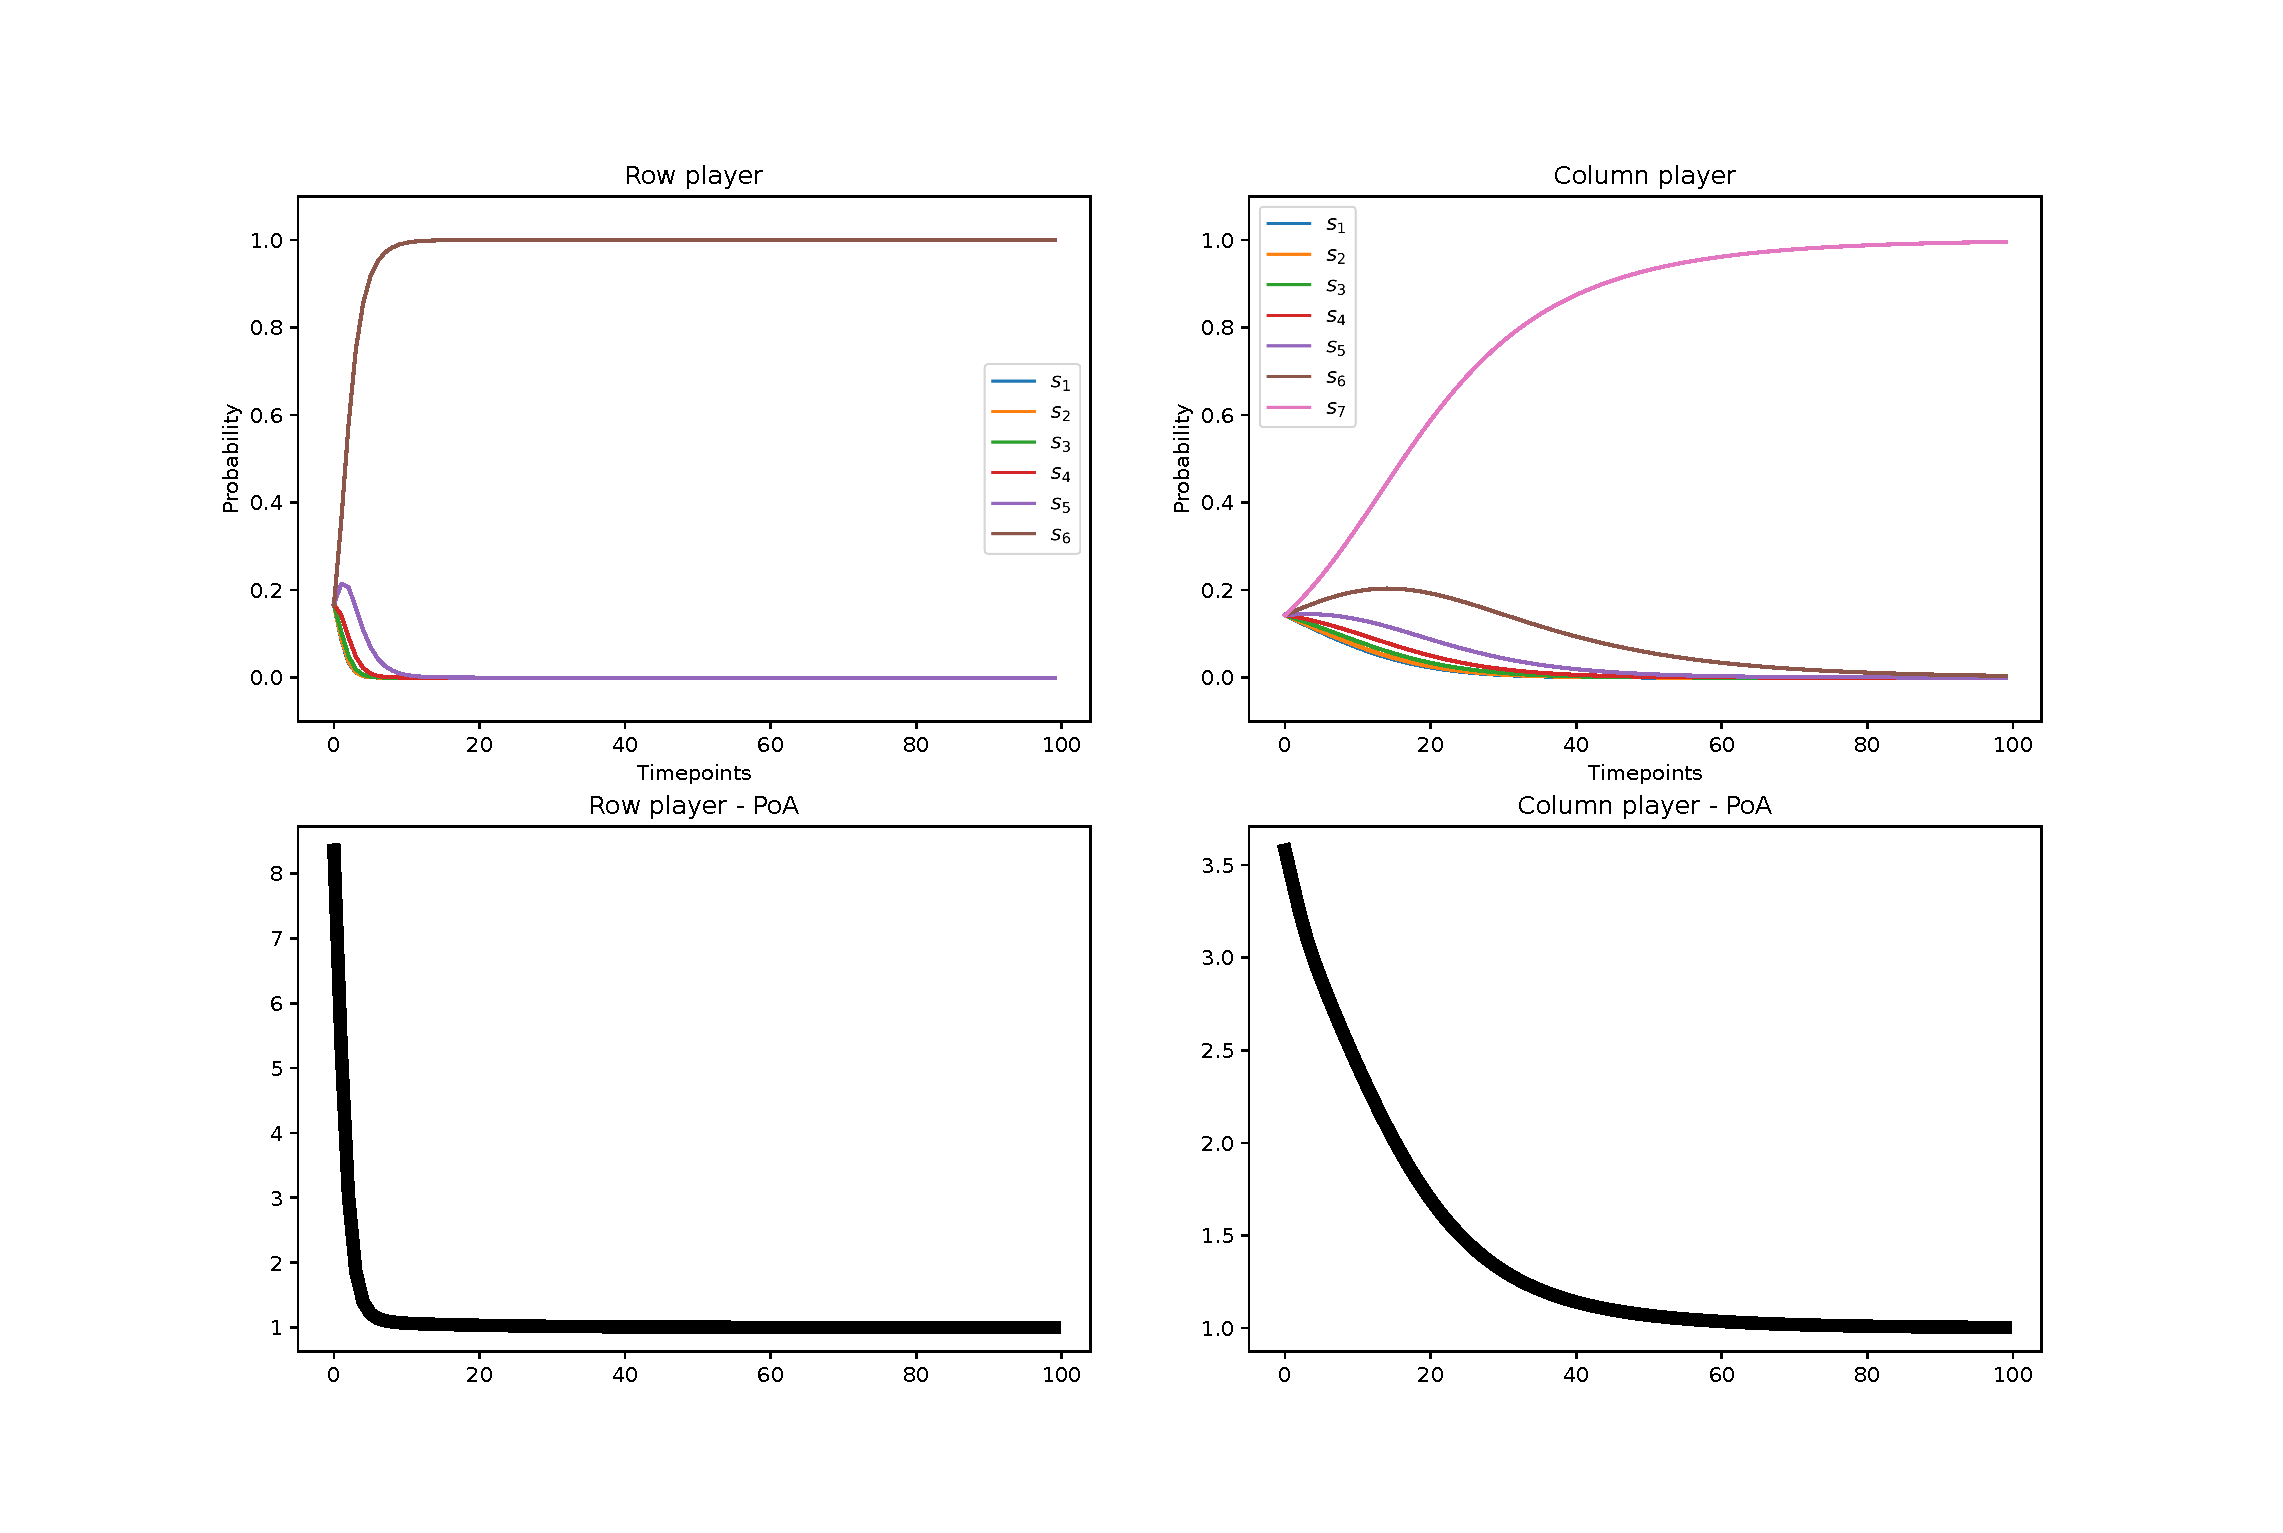
\includegraphics[width=\textwidth, trim = 0 60 0 60, clip]{chapters/00_appendix/02_more_game_results/Bin/poa_ard_other_4.eps}
    \caption{Asymmetric replicator dynamics run and PoA of the game theoretic
    model with parameters: \(\alpha = 1.0, \lambda_2 = 24.0, t = 5.0,
    \lambda_1^{(1)} = 6.0, \lambda_1^{(2)} = 4.5, \mu^{(1)} = 2.0,
    \mu^{(2)} = 3.0, C^{(1)} = 3, C^{(2)} = 2, N^{(1)} = 6, N^{(2)} = 7,
    M^{(1)} = 5, M^{(2)} = 4\).}
    \label{fig:poa_ard_other_4}
\end{figure}
